% !TEX TS-program = pdflatex
% !TEX encoding = UTF-8 Unicode

\documentclass[11pt]{article} 													% use larger type; default would be 10pt
\usepackage[utf8]{inputenc} 													% set input encoding (not needed with XeLaTeX)

%%% PAGE DIMENSIONS ------------------------------------------------------------
\usepackage[top=0.8in, left=1in, right=1in, bottom=1in]{geometry} 			% to change the page dimensions
\geometry{a4paper} 																% or letterpaper (US) or a5paper or....
\usepackage[parfill]{parskip} 													% Activate to begin paragraphs with an empty line rather than an indent

%%% HEADERS & FOOTERS ----------------------------------------------------------
\usepackage{fancyhdr} 															% This should be set AFTER setting up the page geometry
\pagestyle{fancy} 																% options: empty , plain , fancy
\renewcommand{\headrulewidth}{0pt} 												% customise the layout...
\lhead{}\chead{}\rhead{}
\lfoot{}\cfoot{page \thepage}\rfoot{}

%%% SECTION TITLE APPEARANCE ---------------------------------------------------
\usepackage{sectsty}
\allsectionsfont{\sffamily\mdseries\upshape} 									% (See the fntguide.pdf for font help)

%%% PACKAGES -------------------------------------------------------------------
\usepackage[font=small,labelfont=bf,textfont=it]{caption} 						% stylize captions
\usepackage{graphicx} 															% support the \includegraphics command and options
\usepackage{booktabs} 															% for much better looking tables
\usepackage{array} 																% for better arrays (eg matrices) in maths
\usepackage{paralist} 															% very flexible & customisable lists (eg. enumerate/itemize, etc.)
\usepackage{verbatim} 															% adds environment for commenting out blocks of text & for better verbatim
%\usepackage{subfig} 															% make it possible to include more than one captioned figure/table in a single float
\usepackage{mathtools} 															% for math environments like align
\usepackage{amssymb} 															% for symbols like \therefore
\usepackage{verbatim} 															% for including text as appears, verbatim
\usepackage{listings} 															% for including external files as text, eg code
\usepackage{color}																% for coloring of files and images
\usepackage{overpic} 															% for adding annotations to pictures
\usepackage{subcaption} 														% for adding figures side by side (subfigures)
\usepackage{syntonly}															% for checking just the syntax of the document without compiling, use \syntonly

%%% EQUATIONS ------------------------------------------------------------------
\numberwithin{equation}{section} 												% Number equations by section (change for different levels)

%% BIBIOGRAPHY ------------------------------------------------------------------
\usepackage{cite}
\bibliographystyle{unsrt}

%%% ToC (table of contents) APPEARANCE -----------------------------------------
%\usepackage[nottoc,notlof,notlot]{tocbibind} 									% Put the bibliography in the ToC
%\usepackage[titles,subfigure]{tocloft} 										% Alter the style of the Table of Contents
%\renewcommand{\cftsecfont}{\rmfamily\mdseries\upshape}
%\renewcommand{\cftsecpagefont}{\rmfamily\mdseries\upshape} 					% No bold!

%%% NEW COMMANDS ---------------------------------------------------------------
\newcommand{\D}[1]{\,\textrm{d}#1} 												% for integrals
\newcommand{\dx}[2]{\frac{\textrm{d} #1}{\textrm{d} #2}}						% for derivatives
\newcommand{\dd}[2]{\frac{\textrm{d}^2 #1}{\textrm{d} #2^2}}					% for double derivatives
\newcommand{\pd}[2]{\frac{\partial #1}{\partial #2}} 							% for partial derivatives
\newcommand{\pdd}[2]{\frac{\partial^2 #1}{\partial #2^2}} 						% for double partial derivatives
\newcommand{\e}[1]{\text{e}^{#1}} 												% for exponentials
\newcommand{\code}[1]{\texttt{#1}}												% for verbatim code view
\newcommand{\inter}[1]{\shortintertext{#1}}										% shorter version of intertext
\newcommand{\under}[1]{\underline{#1}}											% for vectors etc.

\let\vaccent=\v 																% rename builtin command \v{} to \vaccent{}
\newcommand{\uv}[1]{\ensuremath{\hat{#1}}} 										% for unit vector
\newcommand{\abs}[1]{\left| #1 \right|} 										% for absolute value
\newcommand{\avg}[1]{\left< #1 \right>} 										% for average
\newcommand{\ket}[1]{\left| #1 \right>} 										% for Dirac bras
\newcommand{\bra}[1]{\left< #1 \right|} 										% for Dirac kets
\newcommand{\braket}[2]{\left< #1 \vphantom{#2} \right|
	\left. #2 \vphantom{#1} \right>} 											% for Dirac brackets
\newcommand{\matrixel}[3]{\left< #1 \vphantom{#2#3} \right|
 	#2 \left| #3 \vphantom{#1#2} \right>} 										% for Dirac matrix elements
\newcommand{\grad}[1]{\nabla #1} 												% for gradient
\let\divsymb=\div 																% rename builtin command \div to \divsymb
\renewcommand{\div}[1]{\nabla \cdot #1} 										% for divergence
\newcommand{\curl}[1]{\nabla \times #1} 										% for curl
\let\baraccent=\= 																% rename builtin command \= to \baraccent
\renewcommand{\=}[1]{\stackrel{#1}{=}} 											% for putting numbers above =


%%% Include TIKZ images directly into document ---------------------------------
\usepackage[svgnames]{xcolor}
\usepackage{tikz}
\usetikzlibrary{decorations.markings}
\usetikzlibrary{shapes.geometric}

\newif\iffinal 																	% introduce a switch for draft vs. final document
\finaltrue 																		% use this to compile the final document
\usepackage{tikz}

\iffinal
	\newcommand{\inputTikZ}[1]{%
		\input{#1}%
	}
\else
	\newcommand{\inputTikZ}[1]{%
		\beginpgfgraphicnamed{#1-external}%
		\input{#1}%
		\endpgfgraphicnamed%
	}
\fi

%%% Include svg images directly in document (requires Inkscape) ----------------
\newcommand{\executeiffilenewer}[3]{%
	\ifnum\pdfstrcmp{\pdffilemoddate{#1}}%
		{\pdffilemoddate{#2}}>0%
		{\immediate\write18{#3}}
	\fi
}
\newcommand{\includesvg}[1]{%
	\executeiffilenewer{#1.svg}{#1.pdf}%
	{inkscape -z -D --file=#1.svg --export-pdf=#1.pdf --export-latex}%
	\input{#1.pdf_tex}%
}

%%% PDF LINKS AND STYLE --------------------------------------------------------
\usepackage[unicode=true,
	bookmarks=true,bookmarksnumbered=true,bookmarksopen=true,
	bookmarksopenlevel=2, breaklinks=false,pdfborder={0 0 0},backref=false,
	colorlinks=false] {hyperref} 												% for links in pdf file, no colors
\hypersetup{pdftitle={DOCUMENT NAME},
	pdfauthor={Josh Wainwright}} 												% set name of document and author here


%*******************************************************************************
%******************************** END HEADER ***********************************
%*******************************************************************************
\graphicspath{{./Graphics/}}

\begin{document}
%!TEX root = mainfile.tex
\begin{titlepage}
  \begin{center}
    \vspace*{\fill}

    \centering
    
\includegraphics[scale=1.0]{Logo.pdf}
    \vfill

    \hrule
    {\LARGE\bf Extragalactic Astrophysics and Cosmology\\Cosmic Reionization \\[0.4cm]}
    \hrule

    \vfill
    \large
    School of Physics and Astronomy\\
    University of Birmingham

    \vfill
    { Joe Baumber,
    	James Bryant,
    	Lewis Clegg,
    	Bethany Johnson,
    	Andrew King,
    	Owen McConnell,
    	Catherine McDonald,
    	Michael O'Neill,
    	Jonathan Shepley,
    	Dorothy Stonell,
    	Rahim Topadar,
    	Josh Wainwright\\}
    \vfill

    \vfill
    \textit{Supervisors:} Graham Smith, Alistair Sanderson, Melissa Gillone \\
    		\vfill
    \textit{Date:} March 2013
    \vfill
    \vfill

    \begin{abstract}
        This study deduces that reionization began at a redshift of $z=17.82$ and ended at a redshift of $z=7\pm 1.8$. This is calculated by directly applying the dynamics of star formation and the ionization rate of neutral hydrogen in the Intergalactic Medium. A photometry strategy consisting of 3 multi-band surveys is proposed in order to observe Lyman Break Galaxies across redshifts 6--17. The surveys will locate $100.5\pm37.0$, $138.7\pm 100.6$, $358.1\pm 158.6$ galaxies in redshift ranges 6--8.5, 8.5--10 and 10--17 respectively. These surveys will be completed by the James Webb Space Telescope and Euclid which are planned for launch in the coming decade. A follow up spectroscopy survey will be used to confirm the redshift and properties of 24, 4 and 48 galaxies in these 3 surveys respectively. The spectroscopy will be carried out using James Webb Space Telescope and a combination of single and multi-slit spectroscopy. It is shown that the use of known gravitational lenses, located between redshift 0.5--0.7, is very beneficial for discovering high redshift candidates as it can increase the depth of surveys by up to 3 magnitudes.
    \end{abstract}


  \end{center}
\end{titlepage}

%\thispagestyle{empty}
%\vspace*{\fill}
%\noindent
%\begin{tabular}{ll}
%\end{tabular}

%\cleardoublepage
%\cleardoublepage

\newpage
\tableofcontents
\newpage
%!TEX root = main.tex

\section{Introduction} % (fold)
\label{sec:introduction}
Finite Difference Time Domain is the name given to a technique for modelling the solutions to coupled differential equations, in particular Maxwell's equations for electromagnetism. The technique relies on an algorithm called Yee's algorithm and allows a system to be modelled by calculating the fields for each successive step in time based on the previous value of the fields. The equations are manipulated so that they can be applied with discrete steps in time using central difference approximations.
% section introduction (end)

\section{Maxwell's Equations} % (fold)
\label{sec:maxwell_s_equations}
We shall start with Maxwell's equations for the electromagnetic field, $E$, and the magnetic field, $H$, in free space.
\begin{align}
	\curl{\vec{E}} &= -\mu\cdot\pd{\vec{H}}{t} \\
	\curl{\vec{H}} &= \epsilon\cdot\pd{\vec{E}}{t} \\
	\intertext{Since we are only concerned with the single $x$ dimension, these can be reduced to}
	\curl{\vec{E}} &= -\mu\cdot\dx{\vec{H}}{t} \label{eq:max1}\\
	\curl{\vec{H}} &= \epsilon\cdot\dx{\vec{E}}{t} \label{eq:max2}
\end{align}
These can be written in Cartesian coordinates as follows. Equation \ref{eq:max1} becomes
\begin{align}
	\left( \pd{E_z}{y}-\pd{E_y}{z} \right)\under{i} + \left( \pd{E_x}{z}-\pd{E_z}{x} \right)\under{j} + \left( \pd{E_y}{x}-\pd{E_x}{y} \right)\under{k} &= -\mu\cdot\dx{\vec{H}}{t} \label{eq:max1cart}\\
	\intertext{And equation \ref{eq:max2} is written as}
	\left( \pd{H_z}{y}-\pd{H_y}{z} \right)\under{i} + \left( \pd{H_x}{z}-\pd{H_z}{x} \right)\under{j} + \left( \pd{H_y}{x}-\pd{H_x}{y} \right)\under{k} &= \epsilon\cdot\dx{\vec{E}}{t} \label{eq:max2cart}
\end{align}
For simplicity, we shall consider the Maxwell equations in just 1 dimension. This will mean that the $E$ and $H$ fields vary only in $\hat{z}$ direction and both $\hat{x}$ and $\hat{y}$ are constant. This will simplify the equations greatly, though the theory and application of Yee's algorithm remains very similar. Using this simplification, equation \ref{eq:max1cart} will be written as
\begin{align}
	\pd{E_y}{z}\under{i} - \pd{E_x}{z}\under{j} &= -\mu\cdot\dx{\vec{H}}{t} \label{eq:max1z}\\
	\intertext{and equation \ref{eq:max2cart} as}
	\pd{H_y}{z}\under{i} + \pd{H_x}{z}\under{j} &= \epsilon\cdot\dx{\vec{E}}{t} \label{eq:max2z}
\end{align}

We are now left with two equations, equations \ref{eq:max1z} and \ref{eq:max2z}, that control how $\vec{E}$ and $\vec{H}$ relate to each other both spatially and temporally. This means that, if we have a defined 1 dimensional system that we can specify these fields at a given point, we can calculate the both the fields and see how they vary over time. 

The first equation relates the derivative of the magnetic field, $H$, with respect to time to the derivative of the electric field, $E$, with respect to space. Conversely the second equation relates the derivative of the electric field, $E$, with respect to time to the derivative of the magnetic field, $H$, with respect to space.

These shall be used sequentially, the first to advance the magnetic field, and the second to advance the electric field. Because this deals with a system of differential equations, the calculations can get very complex very quickly. For this reason we shall use an approximation called Yee's algorithm to improve the performance of the model.
% section maxwell_s_equations (end)

%!TEX root = main.tex

\section{Yee's Algorithm} % (fold)
\label{sec:yee_s_algorithm}
Yee's algorithm is a method for solving coupled differential equations, specifically Maxwell's laws, computationally by taking an approximation to the differential as the central differences method.

\subsection{Central Differences Method} % (fold)
\label{sub:central_differences_method}
We shall first look at the approximation to the differential that will be used, the central differences method. 

Consider the Taylor expansion for the function $f(x)$ about the point $x_0\pm\frac{\delta}{2}$,
\begin{align}
	f\left(x_0 + \frac{\delta}{2}\right) &= f(x_0) + \frac{\delta}{2}f'(x_0) + \frac{1}{2!}\left(\frac{\delta}{2}\right)^2f''(x_0) + \frac{1}{3!}\left(\frac{\delta}{2}\right)^3f'''(x_0) + \ldots \\
	f\left(x_0 - \frac{\delta}{2}\right) &= f(x_0) - \frac{\delta}{2}f'(x_0) + \frac{1}{2!}\left(\frac{\delta}{2}\right)^2f''(x_0) - \frac{1}{3!}\left(\frac{\delta}{2}\right)^3f'''(x_0) + \ldots
\end{align}
If we subtract the second from the first, we are left with
\begin{align}
	f\left(x_0 + \frac{\delta}{2}\right) - f\left(x_0 - \frac{\delta}{2}\right) &= \delta f'(x_0) + \frac{2}{3!}\left(\frac{\delta}{2}\right)^3f'''(x_0) + \ldots
\end{align}
This can be rearranged in terms of the derivative, $f'(x_0)$,
\begin{align}
	f'(x_0) = \left.\dx{f(x)}{x}\right|_{x=x_0} &= \frac{f\left(x_0 + \frac{\delta}{2}\right) - f\left(x_0 - \frac{\delta}{2}\right)}{\delta} + O(\delta^2) 
	\intertext{We can approximate this by ignoring the higher order terms, $O(h^2)$,}
	\left.\dx{f(x)}{x}\right|_{x=x_0} &\approx \frac{f\left(x_0 + \frac{\delta}{2}\right) - f\left(x_0 - \frac{\delta}{2}\right)}{\delta} 
\end{align}
This gives us an equation with which we can approximate the gradient at a position by taking the values of the function either side of the point of interest.

There exists three different methods used for finite difference approximations. These are the forward, backward and central differences. We shall use only the central differences method since the other two have inherent issues in some situations if the function to be approximated is not well behaved. The forward approximation method is used for algorithms such as Euler's and the Runge-Kutta methods since these provide the derivative of the function at a future point whereas the backward approximation used the value from a previous iteration when future data is not yet available. The central differences method, since it uses an average of these two is used when the step separation is constant and provides much more accurate approximations, to the order of $O(h^2)$ as opposed to $O(h)$ for the other two methods. 
% subsection central_differences_method (end)

\subsection{Yee's Algorithm} % (fold)
\label{sub:yee_s_algorithm}
The algorithm used to perform finite difference time domain calculations was written by Kane Yee in 1966. It includes several steps:
\begin{enumerate}
	\item Replace all of the derivatives in Ampere's and Faraday's Laws with finite differences and discretise both space and time so that the electric and magnetic fields are staggered spatially and temporally.
	\item Solve these difference equations to obtain a set of ``update equations'' that express the future fields in terms of the past fields that have already been calculated.
	\item Update the magnetic fields to the time corresponding to one step forward in time so that they are known and do the same for the electric fields.
	\item Repeat these, stepping forward in time each time until the required duration has been covered.
\end{enumerate}
% subsection yee_s_algorithm (end)

\subsection{Finite Differences} % (fold)
\label{sub:finite_differences}
We can now replace the differential forms of the equation relating electric and magnetic fields spatially and temporally in equations \ref{eq:max1z} and \ref{eq:max2z} with the finite differences discussed in section \ref{sub:central_differences_method}. The gives a form that relates the electric and magnetic field to the value of the fields one step in time previously. These are shown in equations \ref{eq:updateeqs1} and \ref{eq:updateeqs1}.
\begin{align}
	\frac{E^q_z(m + 1) - E^q_z(m)}{\delta_x} &= \mu \frac{H^{q+\frac{1}{2}}_y\left(m + \frac{1}{2}\right) - H^{q-\frac{1}{2}}_y\left(m - \frac{1}{2}\right)}{\delta_t} \label{eq:updateeqs2}
	\intertext{and}
	\frac{H^{q+\frac{1}{2}}_y\left(m + \frac{1}{2}\right) - H^{q+\frac{1}{2}}_y\left(m-\frac{1}{2}\right)}{\delta_x} &= \epsilon \frac{E^{q+1}_z\left(m\right) - E^q_z\left(m\right)}{\delta_t} \label{eq:updateeqs1}
\end{align}
where $m$ is the spacial step, or the location of the sample being taken, $\delta_x$ is a small difference in space between the points where the samples are taken and likewise, $\delta_t$ is a small step in the temporal direction. The values $m\pm\frac{1}{2}$ and $m\pm 1$ are the values just near to that location, a single step in space or time away, that are used to calculate the approximation.

These equations can be rearranged to give a pair of equations that give the value of the electric or magnetic field in terms of only previous results, so that the wave can be modelled at any point in time given that the wave is known at all points prior to that time. For the electric field, the equation is given in equation \ref{eq:updateE}, and similarly, for the magnetic field in equation \ref{eq:updateM}.
\begin{align}
	E^{q+1}_z(m) &= E^q_z(m) + \frac{\delta_t}{\epsilon\delta_x} \left[ H^{q+\frac{1}{2}}_y\left(m + \tfrac{1}{2}\right) - H^{q+\frac{1}{2}}_y\left(m-\tfrac{1}{2}\right) \right] \label{eq:updateE} \\
	H^{q+\frac{1}{2}}_y(m+\tfrac{1}{2}) &= H^{q-\frac{1}{2}}_y\left(m+\tfrac{1}{2}\right) + \frac{\delta_t}{\mu\delta_x} \Bigg[ E^q_z(m+1) - E^q_z(m) \Bigg] \label{eq:updateM}
\end{align}

These can now be used in a computational simulation of the electromagnetic field.

% subsection finite_differences (end)


% section yee_s_algorithm (end)

%!TEX root = main.tex

\section{Simulations} % (fold)
\label{sec:simulations}

\subsection{Initial Trials with Sinusoidal Waves} % (fold)
\label{ssub:initial_trials_with_sinusoidal_waves}
The simplest, and so easiest to program, wave is the sine wave. Figure \ref{fig:initialsines} shows two examples of a sine wave that is created at the centre of the simulation region. The boundaries are currently totally reflecting and so the waves are reflected back towards the centre where they interfere with each other. The boundaries can be set to absorbing, in which case the wave moves through them and disappears. This has the same appearance as if there were no boundaries and the wave continued to infinity. The relative difference between the magnetic and electric fields is set to a half so that they both can be easily distinguished.
\begin{figure}[ht]
        \centering
        \begin{subfigure}[ht]{0.45\textwidth}
                \centering
                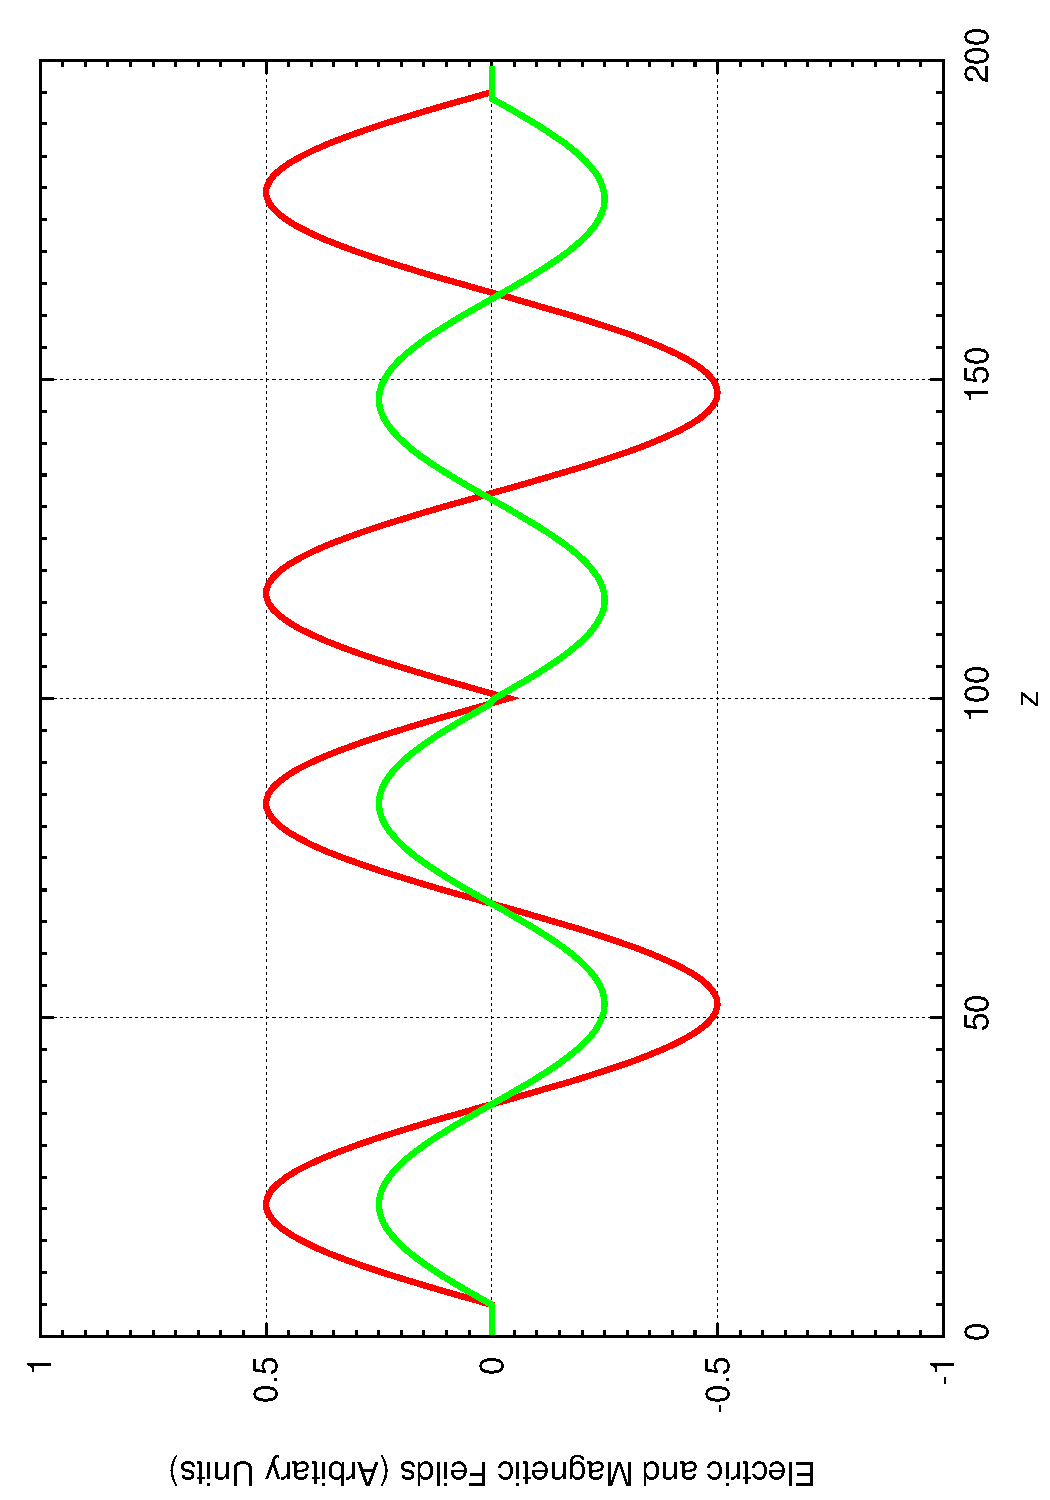
\includegraphics[angle=270, width=\textwidth]{infsine.pdf}
        \end{subfigure}%
        ~
        \begin{subfigure}[ht]{0.45\textwidth}
                \centering
                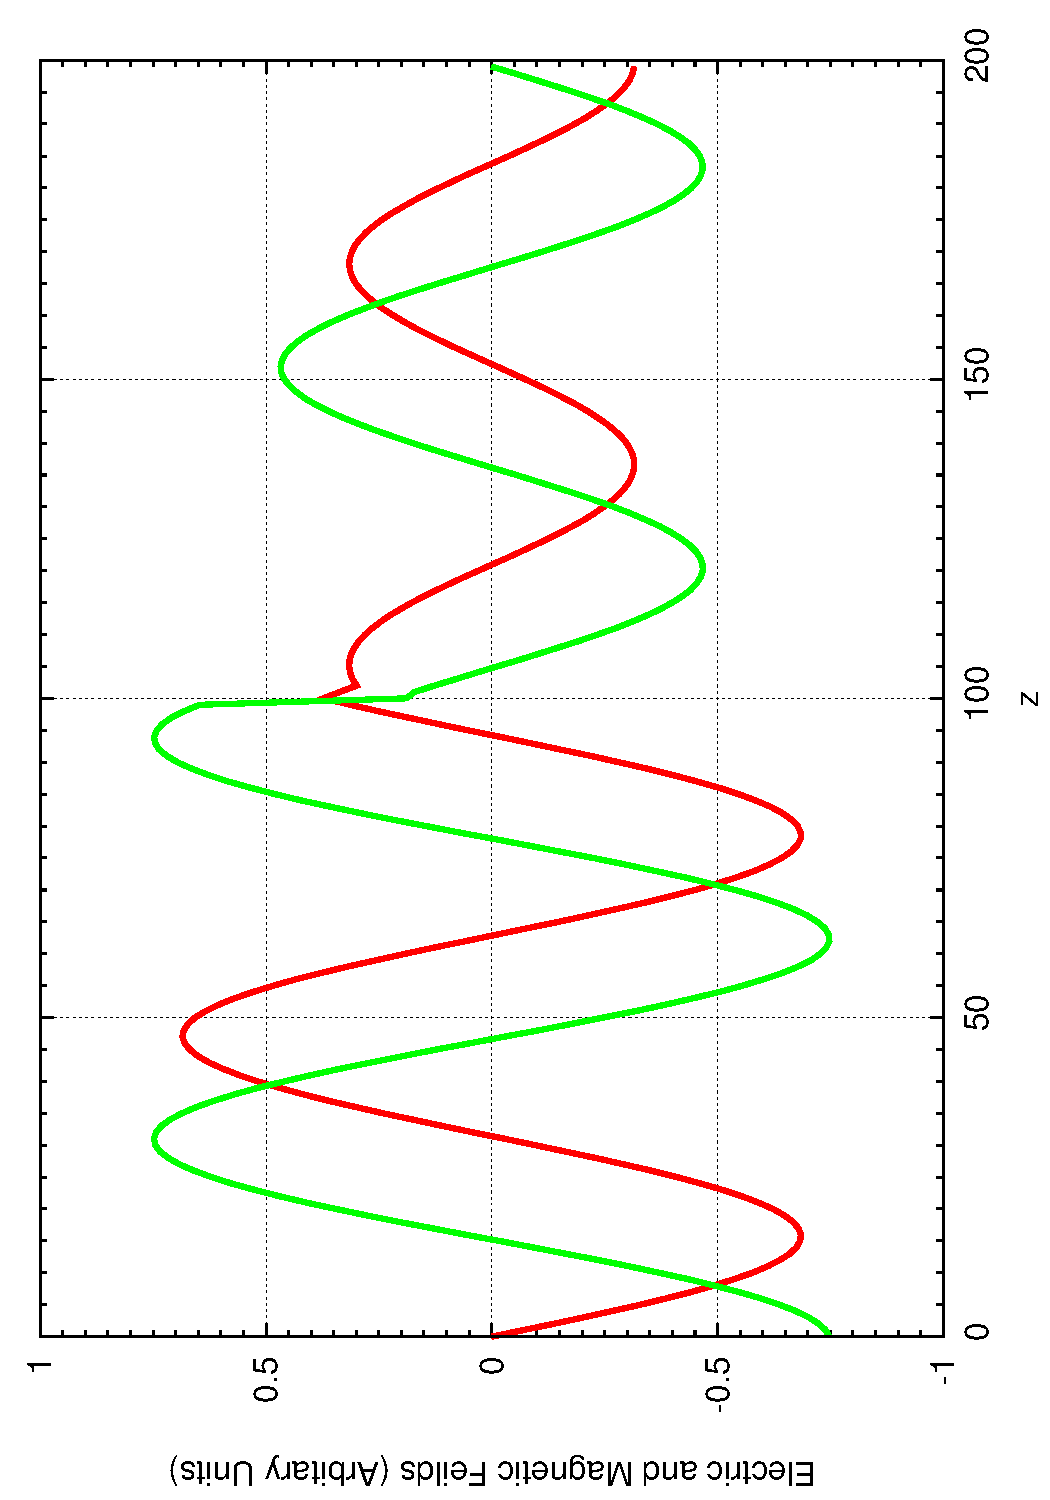
\includegraphics[angle=270, width=\textwidth]{boundsine.pdf}
        \end{subfigure}
        \caption{Two frames from a sine wave that is created in the centre of the region. The first wave is a simple sine wave in a system with perfectly absorbing boundaries. The seconds shows the same sine wave, but with reflecting boundaries and given more time to evolve.}\label{fig:initialsines}
\end{figure}

Since the source is continually creating the wave, the amplitude of the waves in the bounded case increases as the existing reflected waves interfere with the newly created ones. 
% subsubsection initial_trials_with_sinusoidal_waves (end)

\subsection{Initial Trials with Gaussian Pulse} % (fold)
\label{sub:initial_trials_with_gaussian_pulse}
A slightly more complex function is the Gaussian function that generates a pulse of a specified width and height. This function has the equation
\begin{align}
        f(x) &= a\cdot\e{-\frac{(x-b)^2}{2c^2}} \label{eq:gaussian}
\end{align}
where $a$, $b$ and $c$ are constants that determine the width, height and position of the function.

Three frames showing the start of the wave are shown in figure \ref{fig:initialguass}. This time the wave is created at the origin, again the boundaries are totally absorbing. A point to note is that, though in this case, the magnetics field, green, is negative and the electric field, red, is positive, these relations really have no physical meaning. This representation is used so that the relative position of the two waves can be seen. In reality, the two components of the wave will be at $90^{\circ}$ to each other so that one is in the $x$-axis and the other in the $y$-axis. The relative signs of the wave with respect to the other depends on the direction of travel, as defined by the ``right hand rule''. Later, the wave is represented in three dimensions where the relation between the two is more physically accurate.
\begin{figure}[ht]
        \centering
        \begin{subfigure}[ht]{0.45\textwidth}
                \centering
                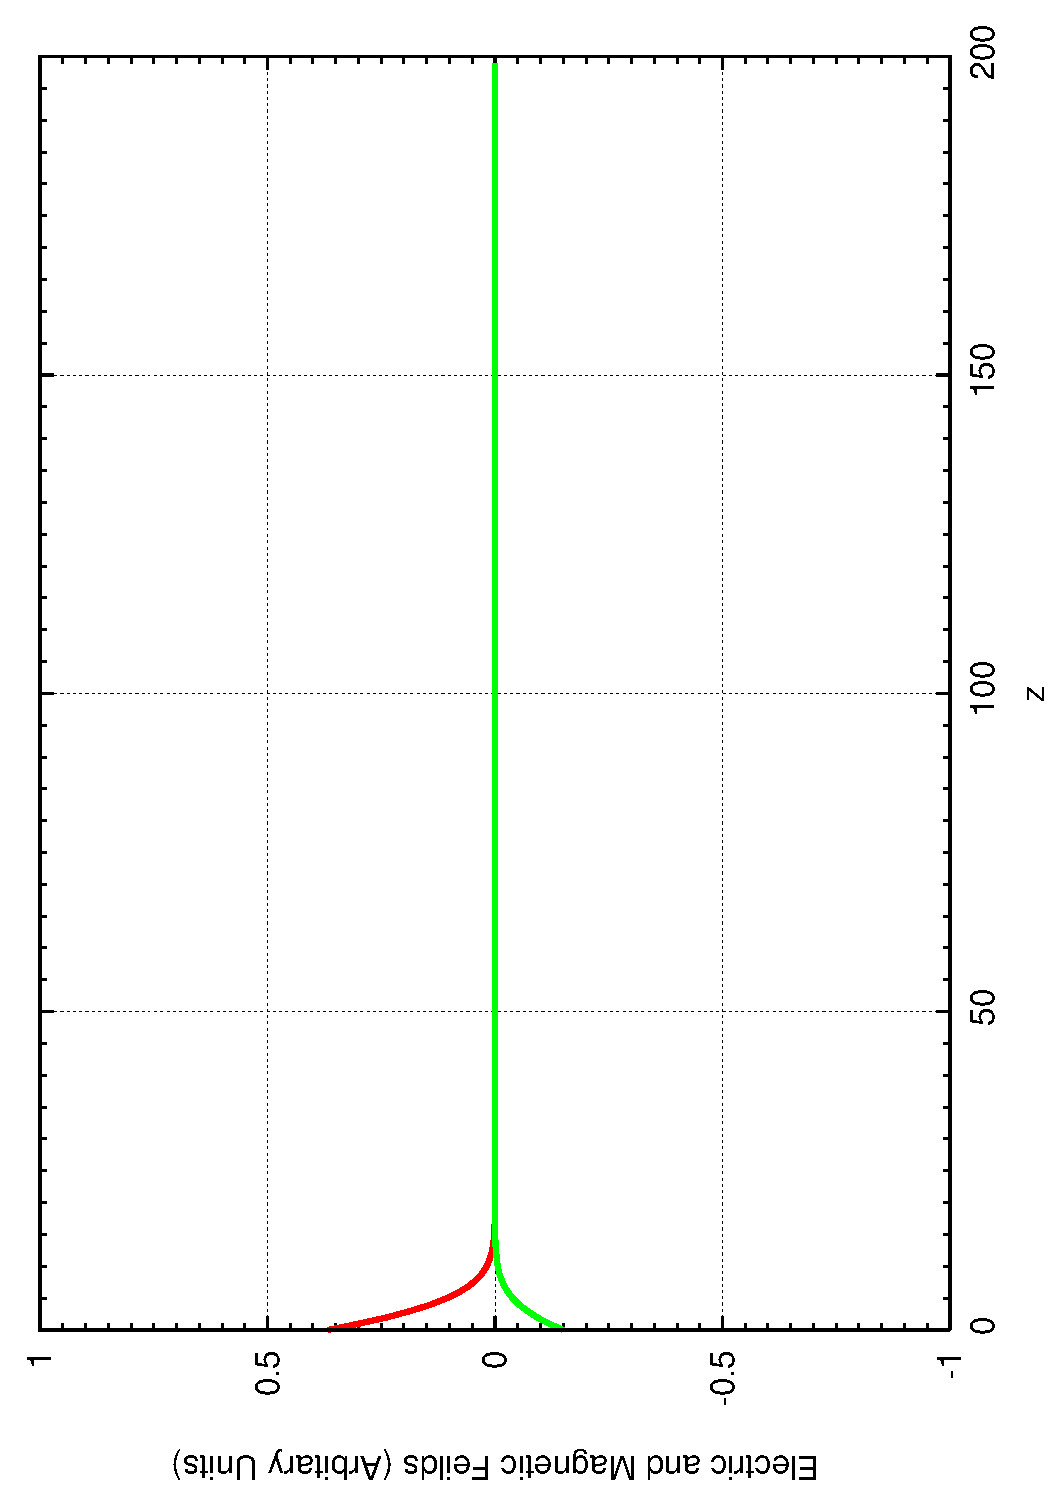
\includegraphics[angle=270, width=\textwidth]{initialguass1.pdf}
        \end{subfigure}%
        ~
        \begin{subfigure}[ht]{0.45\textwidth}
                \centering
                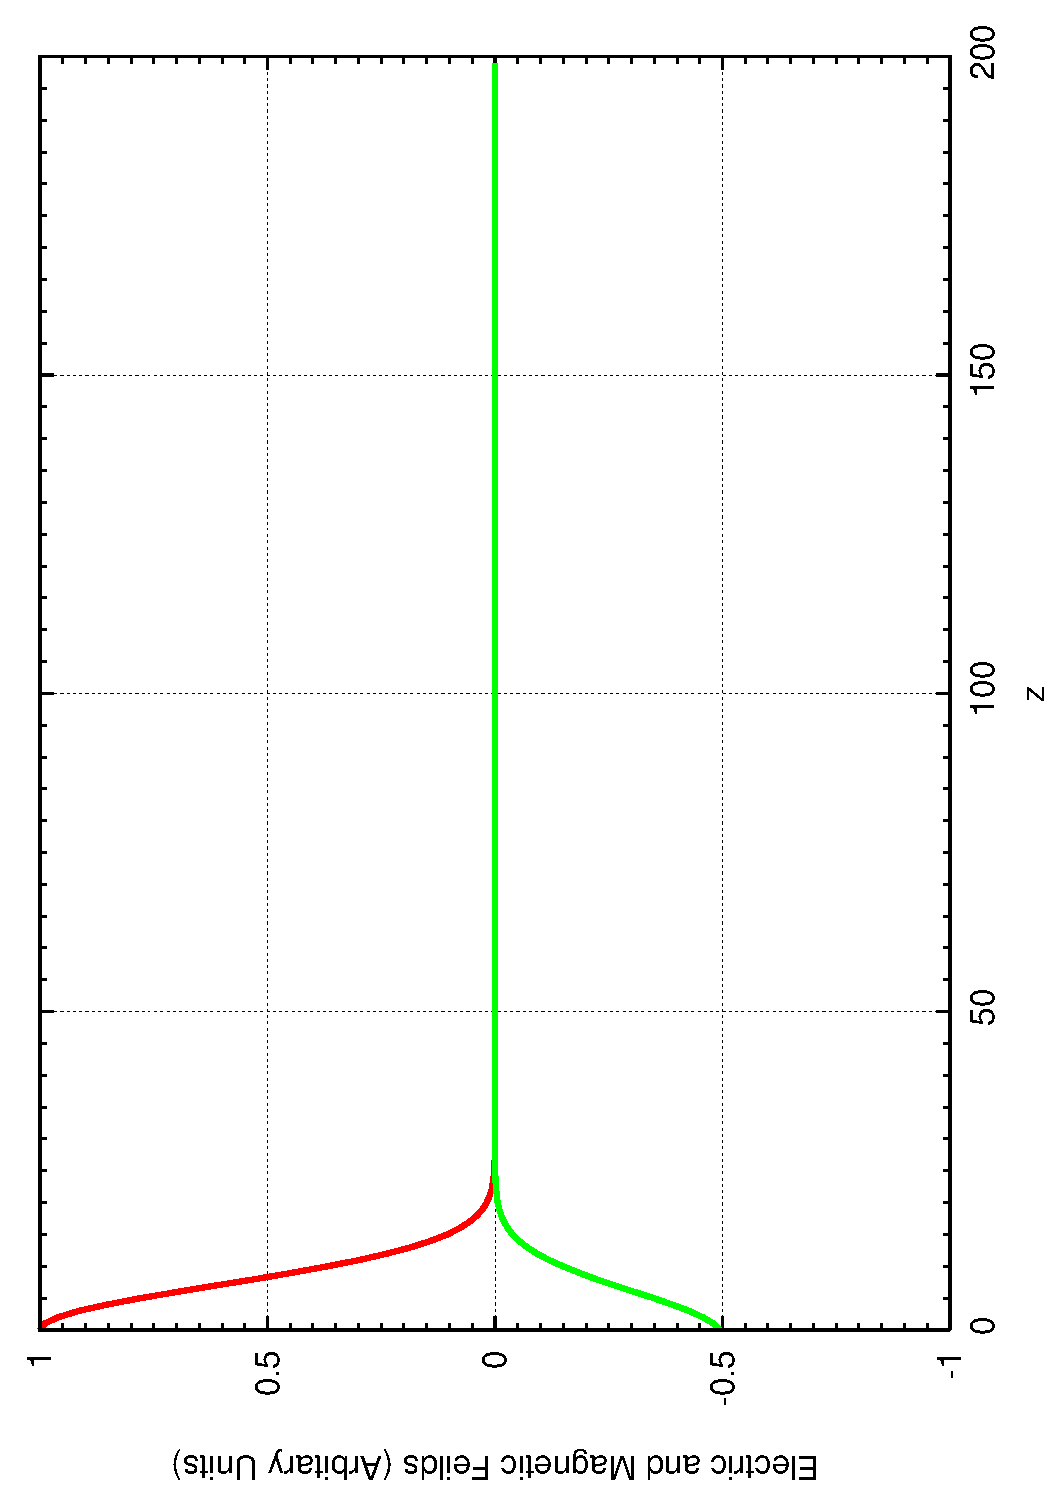
\includegraphics[angle=270, width=\textwidth]{initialguass2.pdf}
        \end{subfigure}

        \begin{subfigure}[ht]{0.45\textwidth}
                \centering
                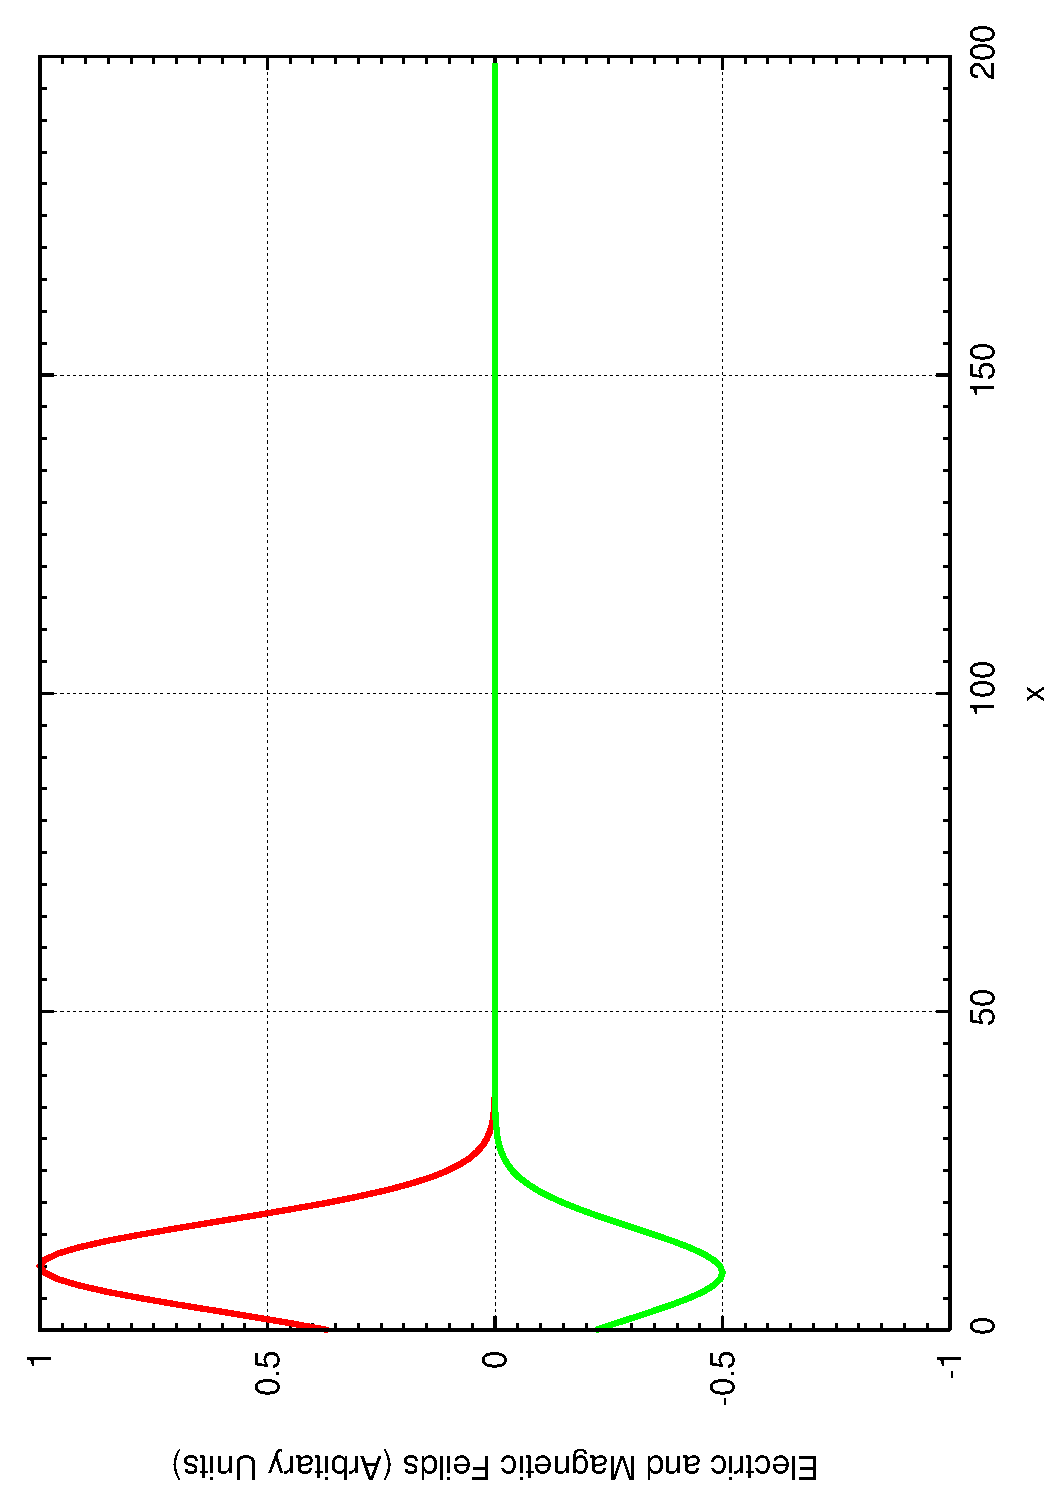
\includegraphics[angle=270, width=\textwidth]{initialguass3.pdf}
        \end{subfigure}
        ~
        \begin{subfigure}[ht]{0.45\textwidth}
                \centering
                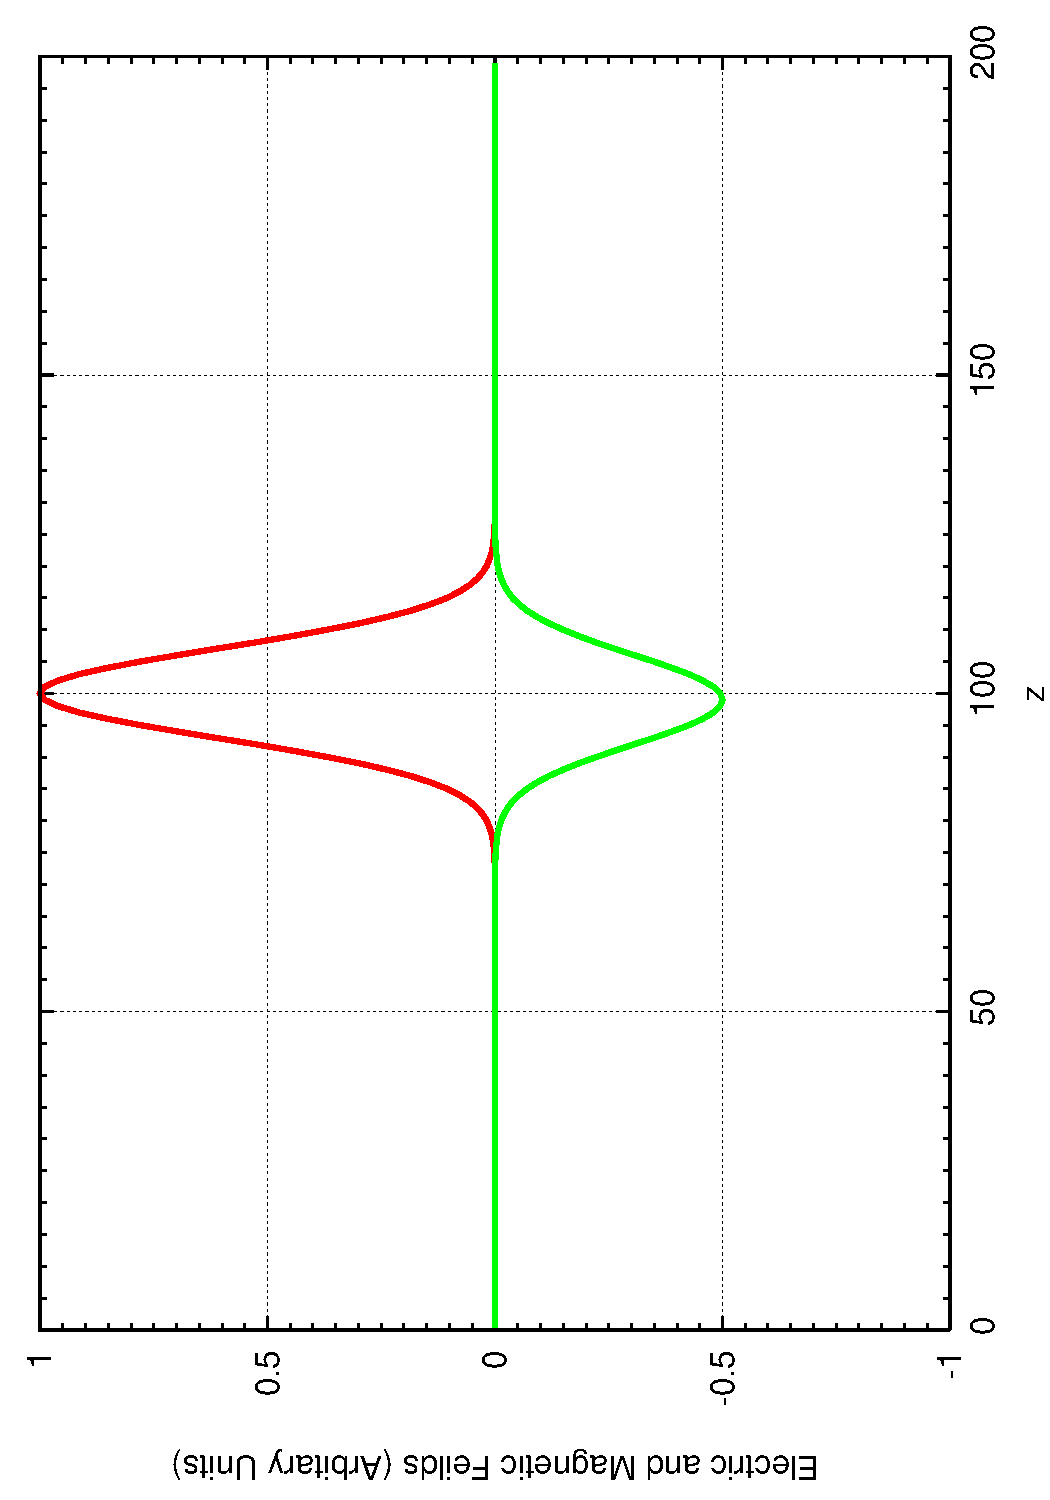
\includegraphics[angle=270, width=\textwidth]{initialguass4.pdf}
        \end{subfigure}
        \caption{An image of three frames each 10 frames apart showing the development and the start of propagation of a Gaussian shaped pulse, as well as a frame showing the pulse as it traverses the simulation area.}\label{fig:initialguass}
\end{figure}

This wave can be seeded at any point in the $z$ axis within the simulation area, $[0,200]$, as specified by the user. If the starting point for the wave is within the area, as opposed to at either edge, then two waves are generated and propagate in both directions away from the centre, figure \ref{fig:initialcenter}.
\begin{figure}[ht]
        \centering
        \begin{subfigure}[ht]{0.45\textwidth}
                \centering
                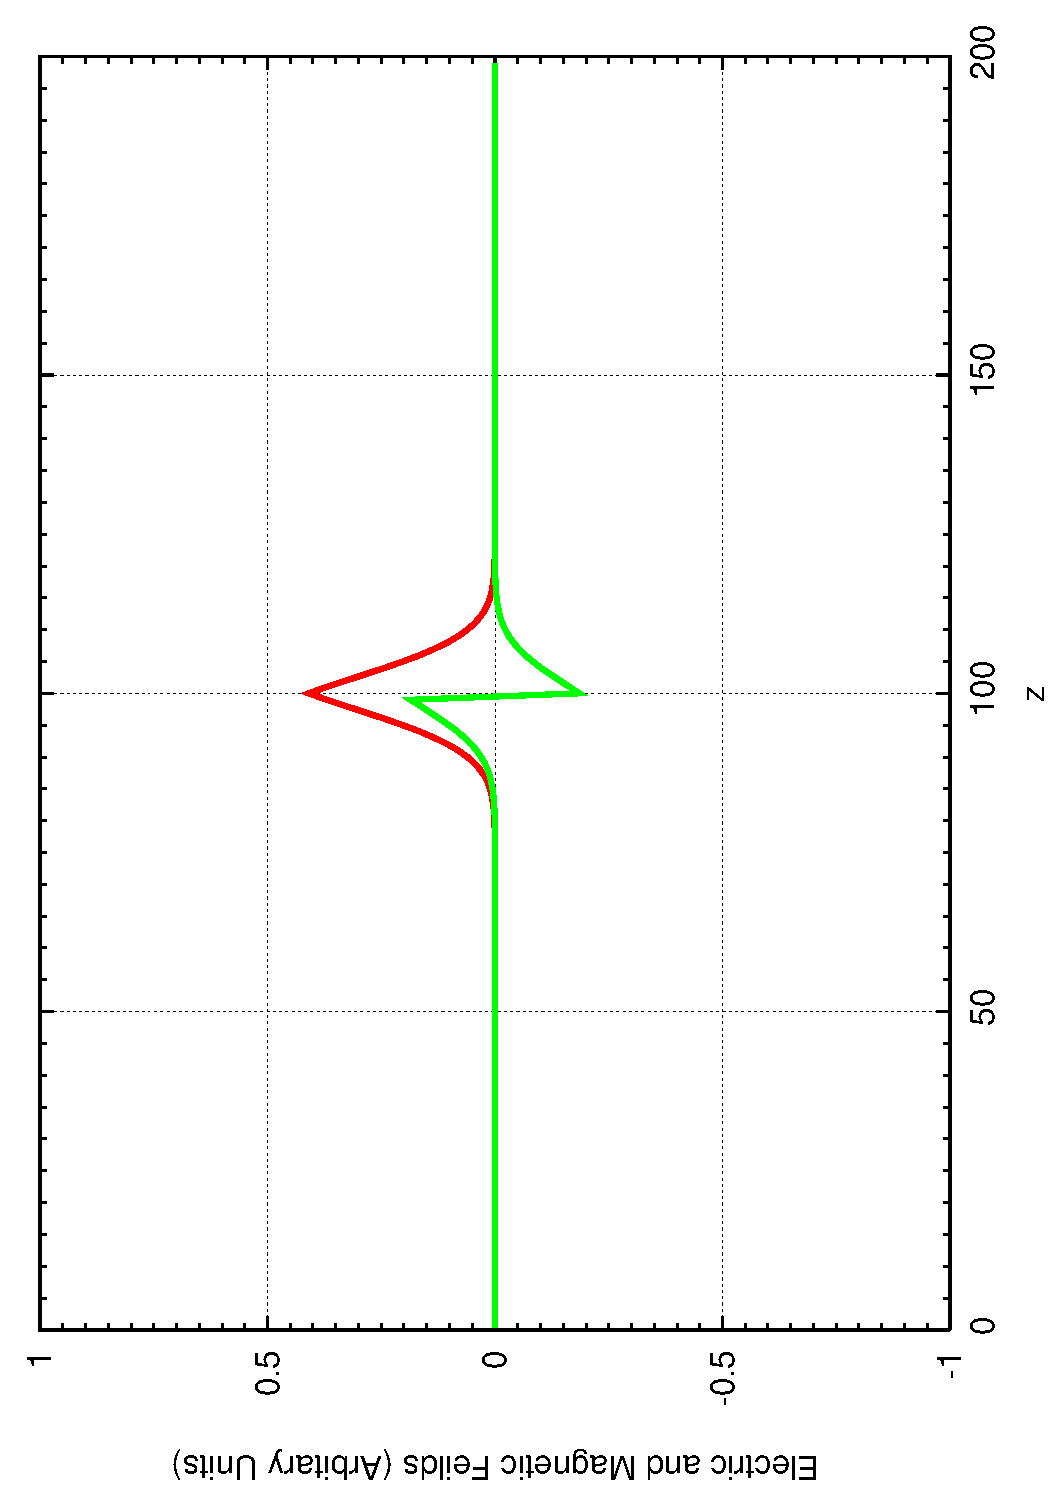
\includegraphics[angle=270, width=\textwidth]{centerseed1.pdf}
        \end{subfigure}%
        ~
        \begin{subfigure}[ht]{0.45\textwidth}
                \centering
                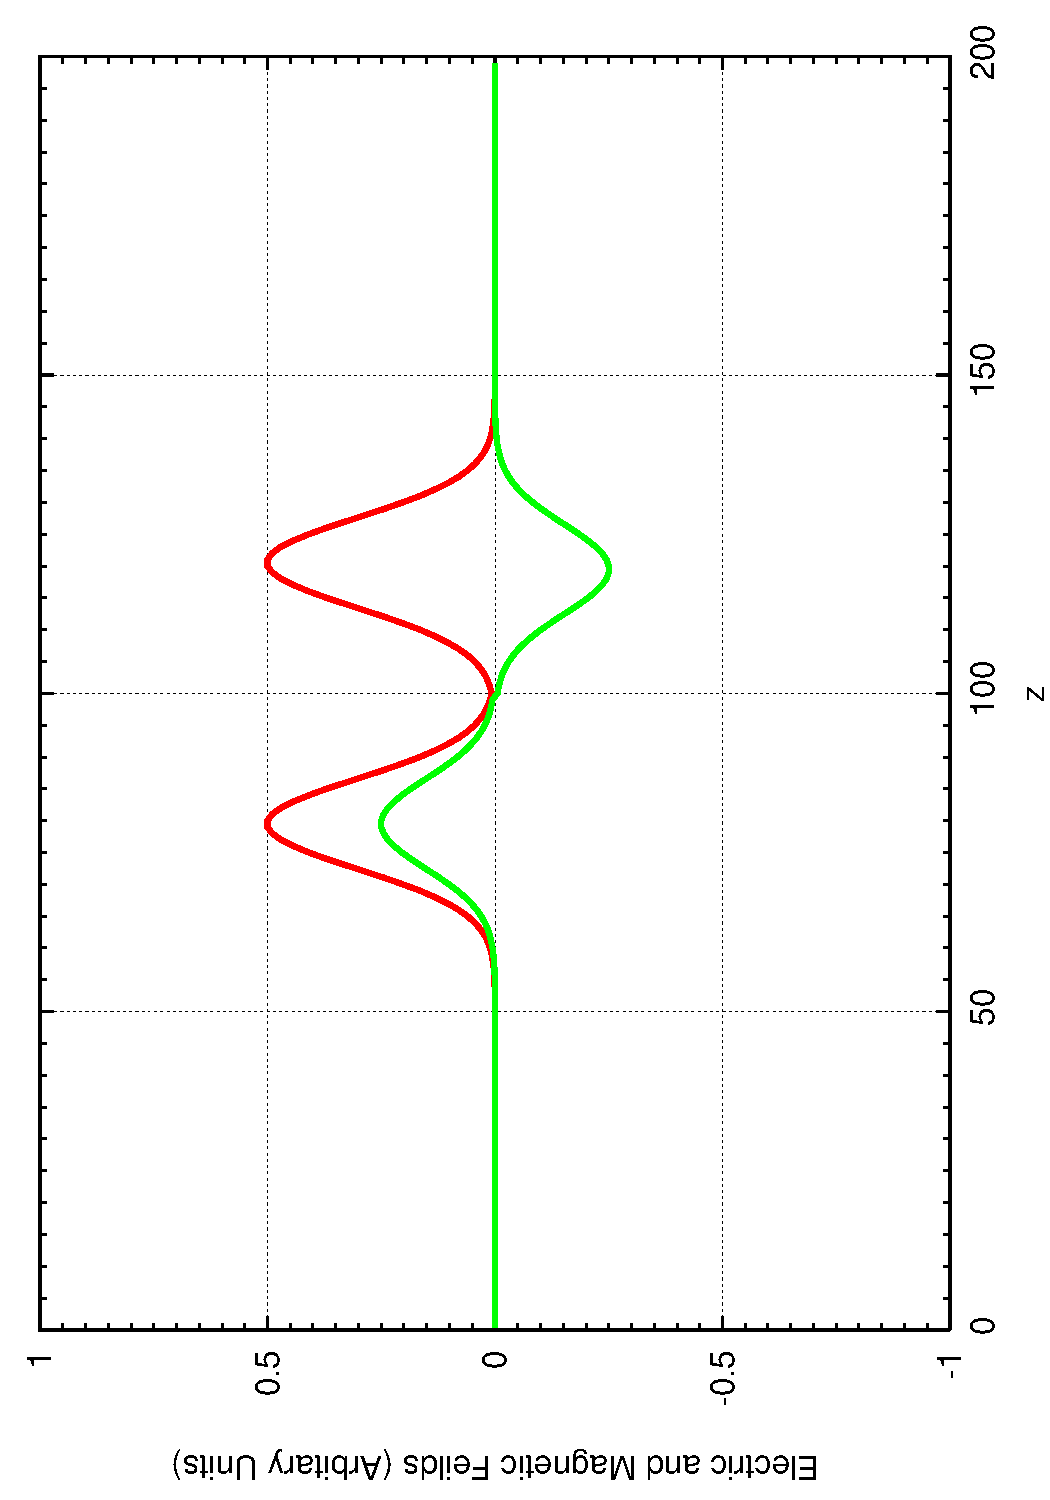
\includegraphics[angle=270, width=\textwidth]{centerseed2.pdf}
        \end{subfigure}
        \caption{Two frames from a wave that is created in the centre of the region. The seed point creates two pulses that move away from each other. The amplitude is set to one half of previous so that when they interact after colliding with the walls, the resulting peak stays within the graphing area.}\label{fig:initialcenter}
\end{figure}

Figure \ref{fig:initialcenter} shows clearly the difference in the sign of the magnetic wave, which is calculated from the electric, when moving in opposite directions. The discontinuity in the magnetic wave in the first image is due to the discontinuity of the first derivative of the electric wave when it is created. 
% subsection initial_trials_with_gaussian_pulse (end)

\subsection{Dielectric Material} % (fold)
\label{sub:dielectirc_material}
A dielectric material is an electrical insulator that can be polarized by an electric field. This means that when an electric field enters a dielectric material, some of the energy is lost to the material and so the amplitude of the wave decreases. 

\subsubsection{Non-Lossy Material} % (fold)
\label{ssub:non_lossy_material}
We shall first consider the case where a dielectric medium is placed in the simulation area which has a finite, non-zero permittivity, but is not lossy. This means that the material will cause an incident wave to be partly transmitted, but also partly reflected. 

The absolute permittivity of a dielectric material is a measure of the resistance felt when forming an electric field inside a conducting material. It is given by equation \ref{eq:absepsilon}.
\begin{align}
    \epsilon &= \epsilon_r \epsilon_0 \label{eq:absepsilon}
\end{align}
where $\epsilon_0=8.85419\times 10^{-12}\,\text{Fm}^{-1}$ is the permittivity of free space and $\epsilon_r$ is the relative permittivity of the material in question. It is this value that shall be changed for the dielectric in the simulation. A value of $\epsilon_r=10.0$ is used in the simulation which is roughly comparable to that of graphite or salt (NaCl). 

If a dielectric is placed in the simulation area, the wave will be incident on it and decrease in amplitude as it travels trough. In order to conserve the energy and momentum of the wave, part of the wave is reflected back from the boundary between free space and the dielectric. The ratio of the transmitted wave to the reflected wave is given by equation \ref{eq:reflectioncoeff}.
\begin{align}
    C &= \frac{R}{T}, \label{eq:reflectioncoeff}
\end{align}
where $C$ is the reflection coefficient of the reflected wave of amplitude $R$, which is produced when an initial wave hits a boundary, and the transmitted wave with amplitude $T$, which travels through the boundary. This is equal to 
\begin{align}
    C &= \left| \frac{n_1\cos\theta_i - n_2\cos\theta_t}{n_1\cos\theta_i + n_2\cos\theta_t}\right|^2 
    \intertext{Using Snell's law, $\frac{\sin\theta_i}{\sin\theta_t} = \frac{n_2}{n_1}$, this can be written as}
    C &= \left| \frac{n_1\cos\theta_i - n_2\sqrt{1-\left( \frac{n_1}{n_2}\sin\theta_i \right)^2}}{n_1\cos\theta_i + n_2\sqrt{1-\left( \frac{n_1}{n_2}\sin\theta_i \right)^2}} \right|^2
    \intertext{Since, in this situation, the waves are approaching the boundary at $90^\circ$, this reduces to}
    C &= \left| \frac{n_1 - n_2}{n_1 + n_2} \right|^2
\end{align}

An example, again using the Gaussian function, can be seen in figure \ref{fig:dielectricgauss}. Here, free space is represented by a white background and the dielectric is the grey shaded area.
\begin{figure}[ht]
        \centering
        \begin{subfigure}[ht]{0.45\textwidth}
                \centering
                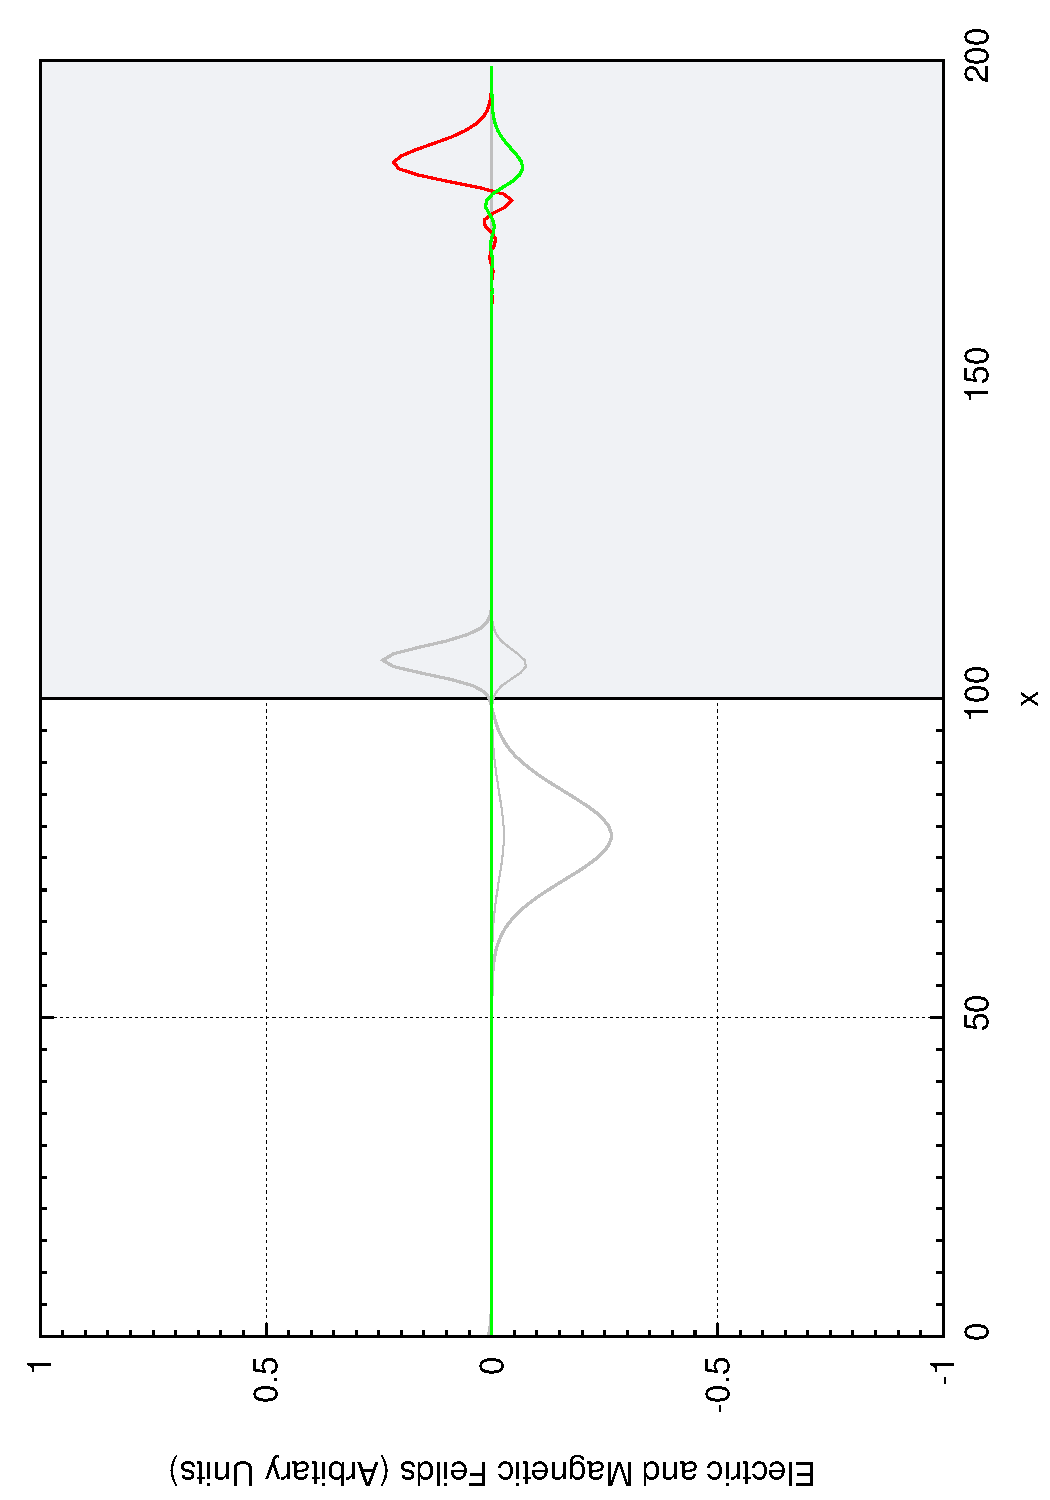
\includegraphics[angle=270, width=\textwidth]{dielectricdouble.pdf}
        \end{subfigure}%
        ~
        \begin{subfigure}[ht]{0.45\textwidth}
                \centering
                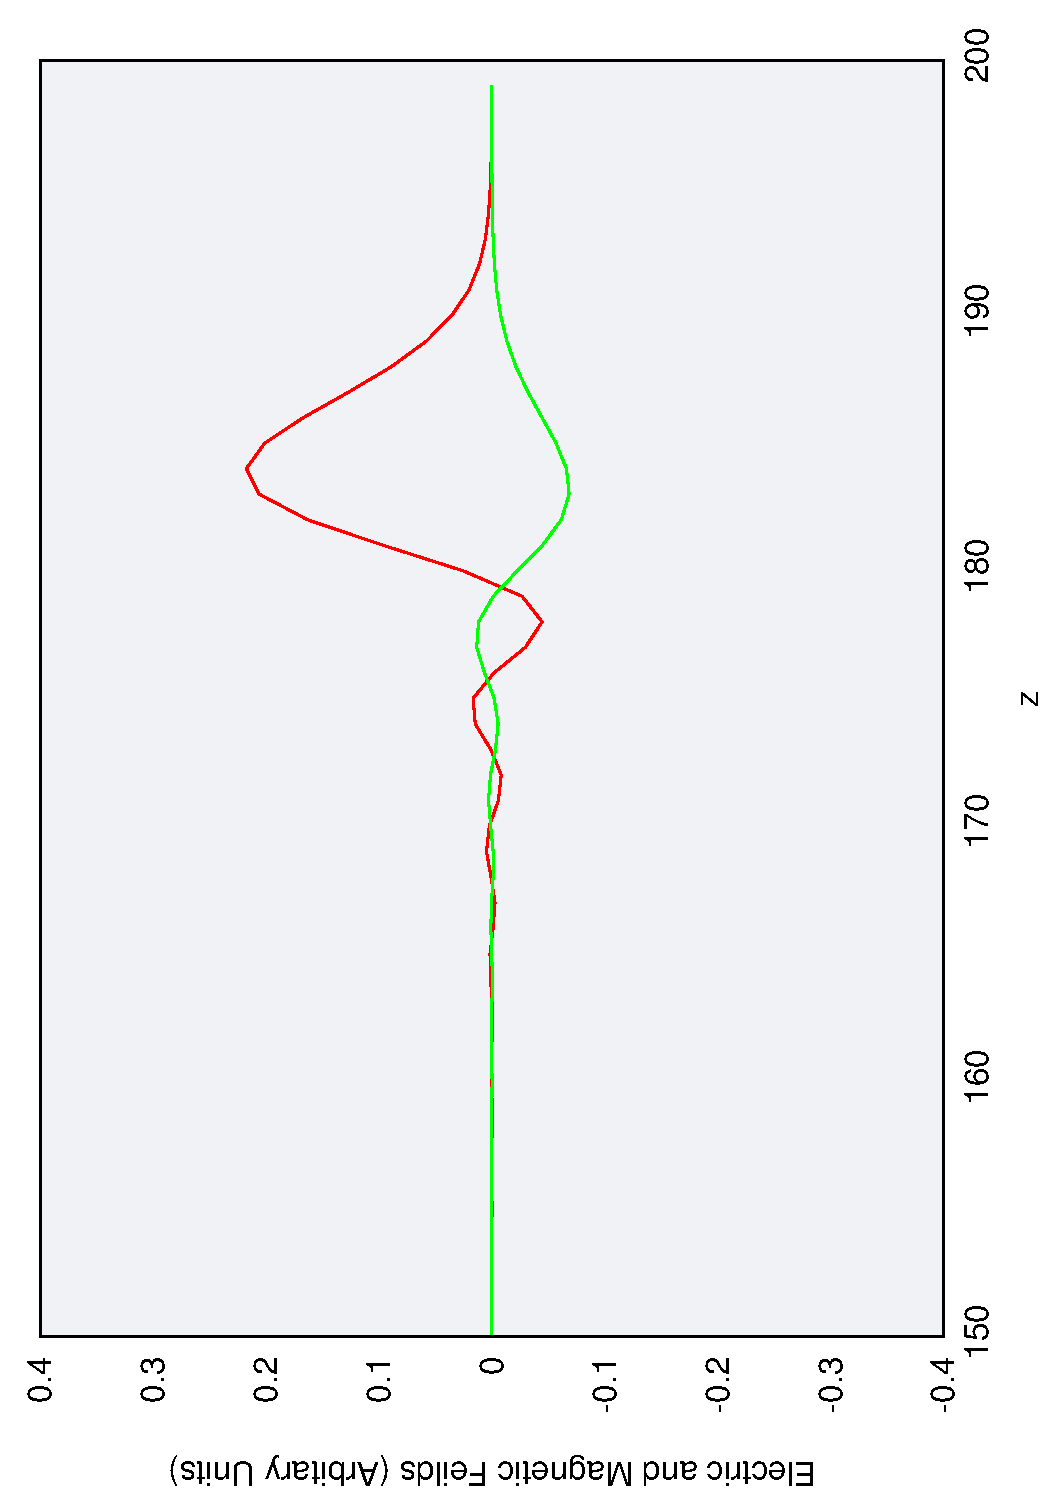
\includegraphics[angle=270, width=\textwidth]{gaussnoise1b.pdf}
        \end{subfigure}
        \caption{A dielectric is now added to the simulation area. This dielectric is not lossy , so the propagating wave does not loose any energy, but it has a finite permittivity of 10 so that the amplitude is decreased when the wave is incident on the dielectric boundary. Part of the wave is reflected back and some propagates through the material. The first image shows the wave just after it has hit the boundary where a reflected and transmitted wave of equal magnitude but opposite sign and different width are seen. And the second image shows a larger image of the transmitted wave as it propagates through the medium. The departure from a true Gaussian function can be seen clearly here as well as the limitation of the simulation in the straight lines that make up the curve.}\label{fig:dielectricgauss}
\end{figure}

The second diagram in figure \ref{fig:dielectricgauss} shows the wave once it has propagated a significant distance through the dielectric material. This wave resembles a sinusoidal pulse instead of the simple Gaussian function since there are extra periods to the function behind the main peak. These smaller peaks are not physical and are instead an artefact of computation.

These peaks are due to the temporal/spacial time step of the simulation being relatively large. This can be demonstrated by increasing the frequency of a sine wave, while keeping other factors constant. Figure \ref{fig:highfreqsine} shows a series of sine wave with increasing frequency.
\begin{figure}[ht]
        \centering
        \begin{subfigure}[ht]{0.45\textwidth}
                \centering
                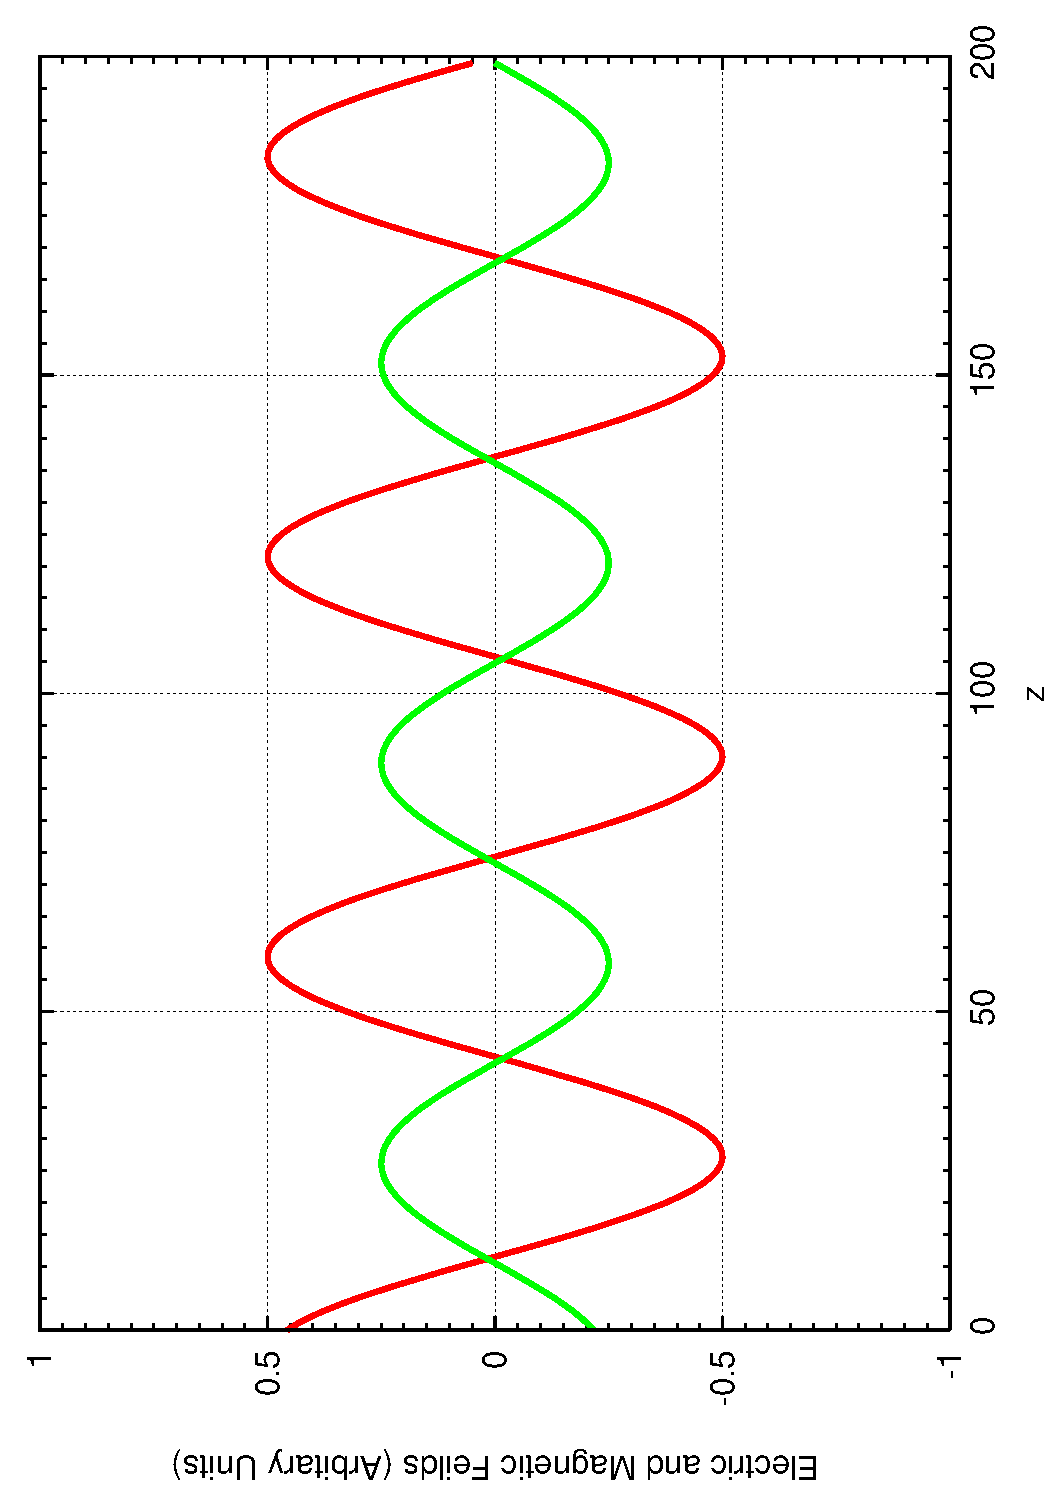
\includegraphics[angle=270, width=\textwidth]{highfreqsine1.pdf}
        \end{subfigure}%
        ~
        \begin{subfigure}[ht]{0.45\textwidth}
                \centering
                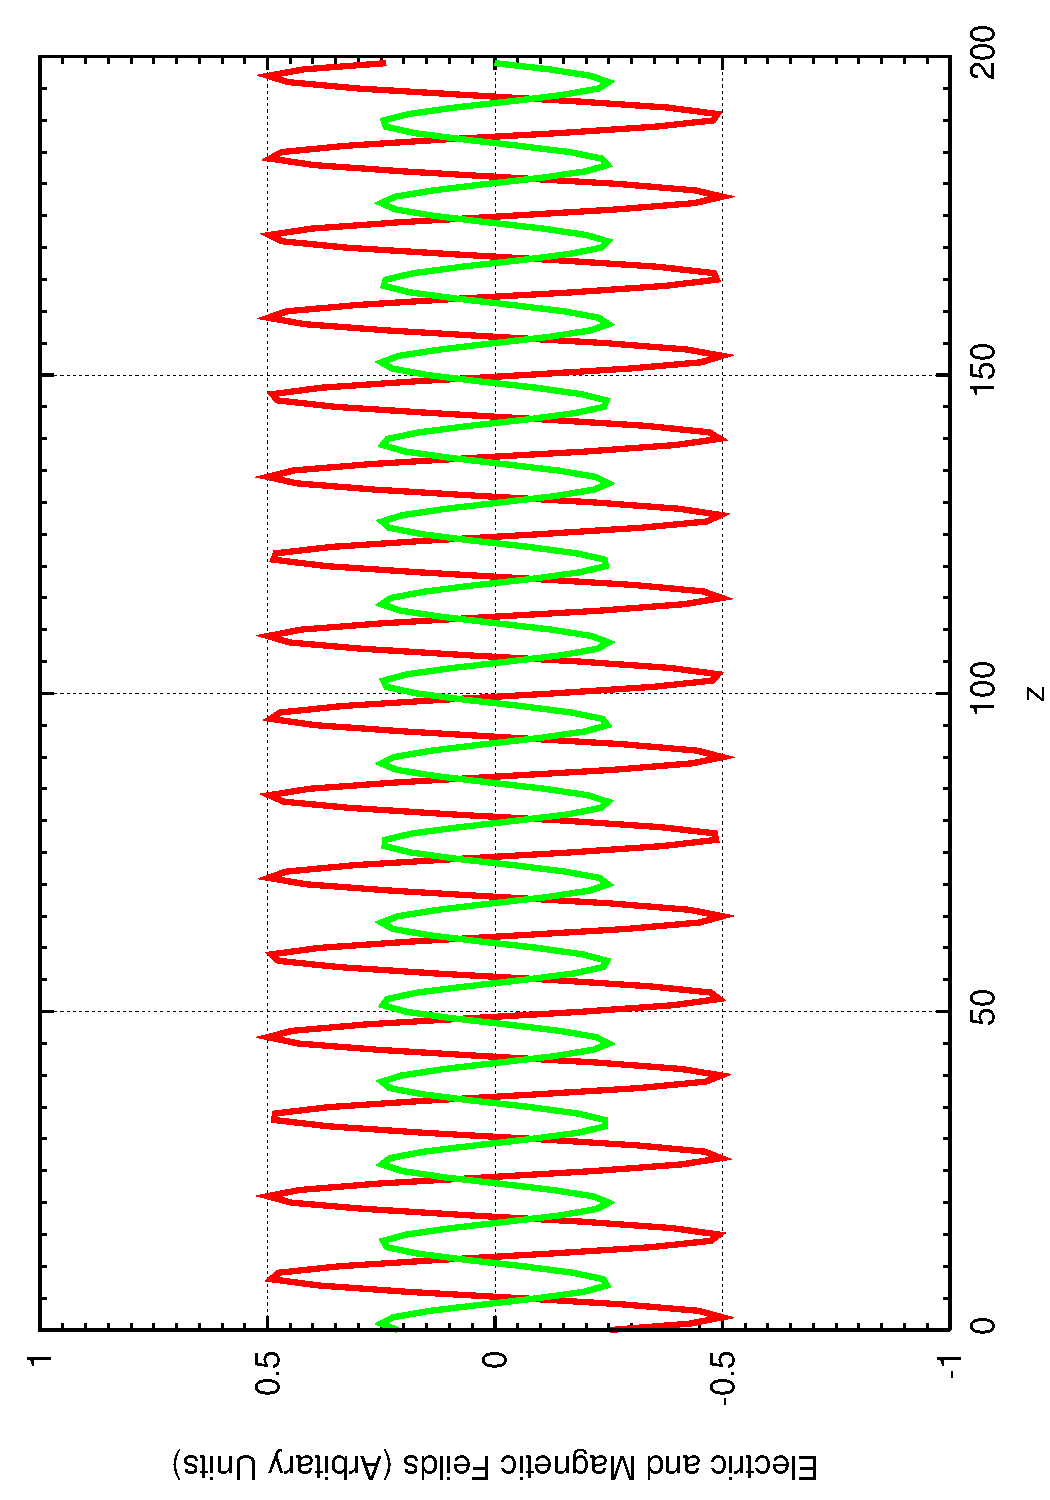
\includegraphics[angle=270, width=\textwidth]{highfreqsine2.pdf}
        \end{subfigure}

        \begin{subfigure}[ht]{0.45\textwidth}
                \centering
                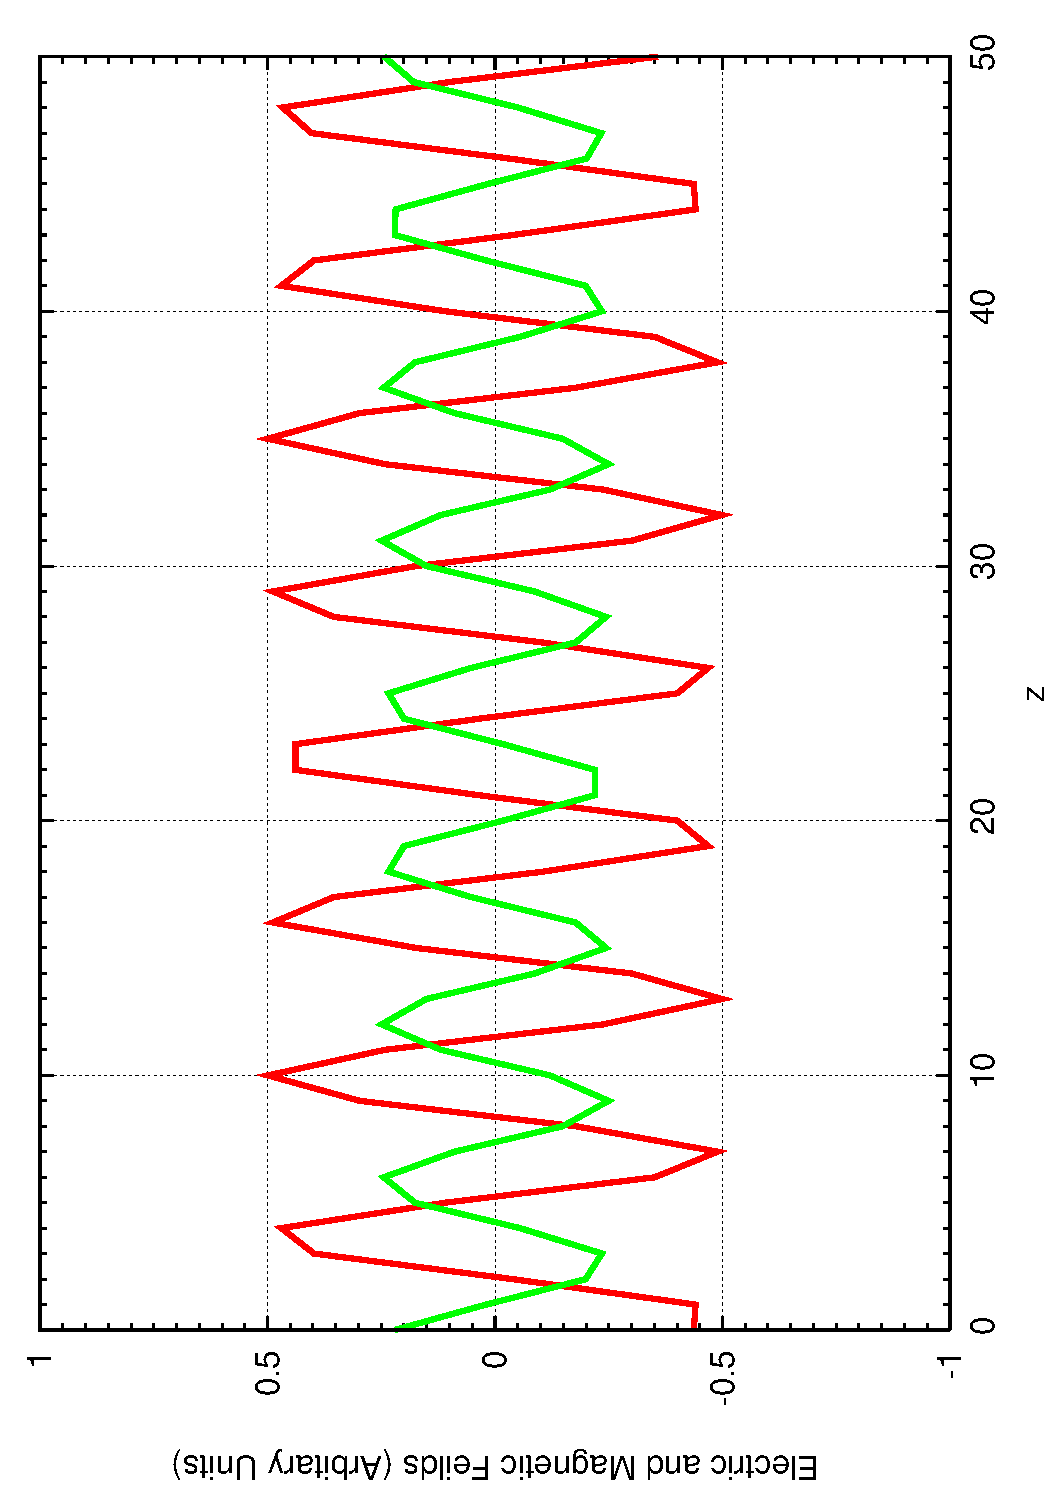
\includegraphics[angle=270, width=\textwidth]{highfreqsine3.pdf}
        \end{subfigure}
        ~
        \begin{subfigure}[ht]{0.45\textwidth}
                \centering
                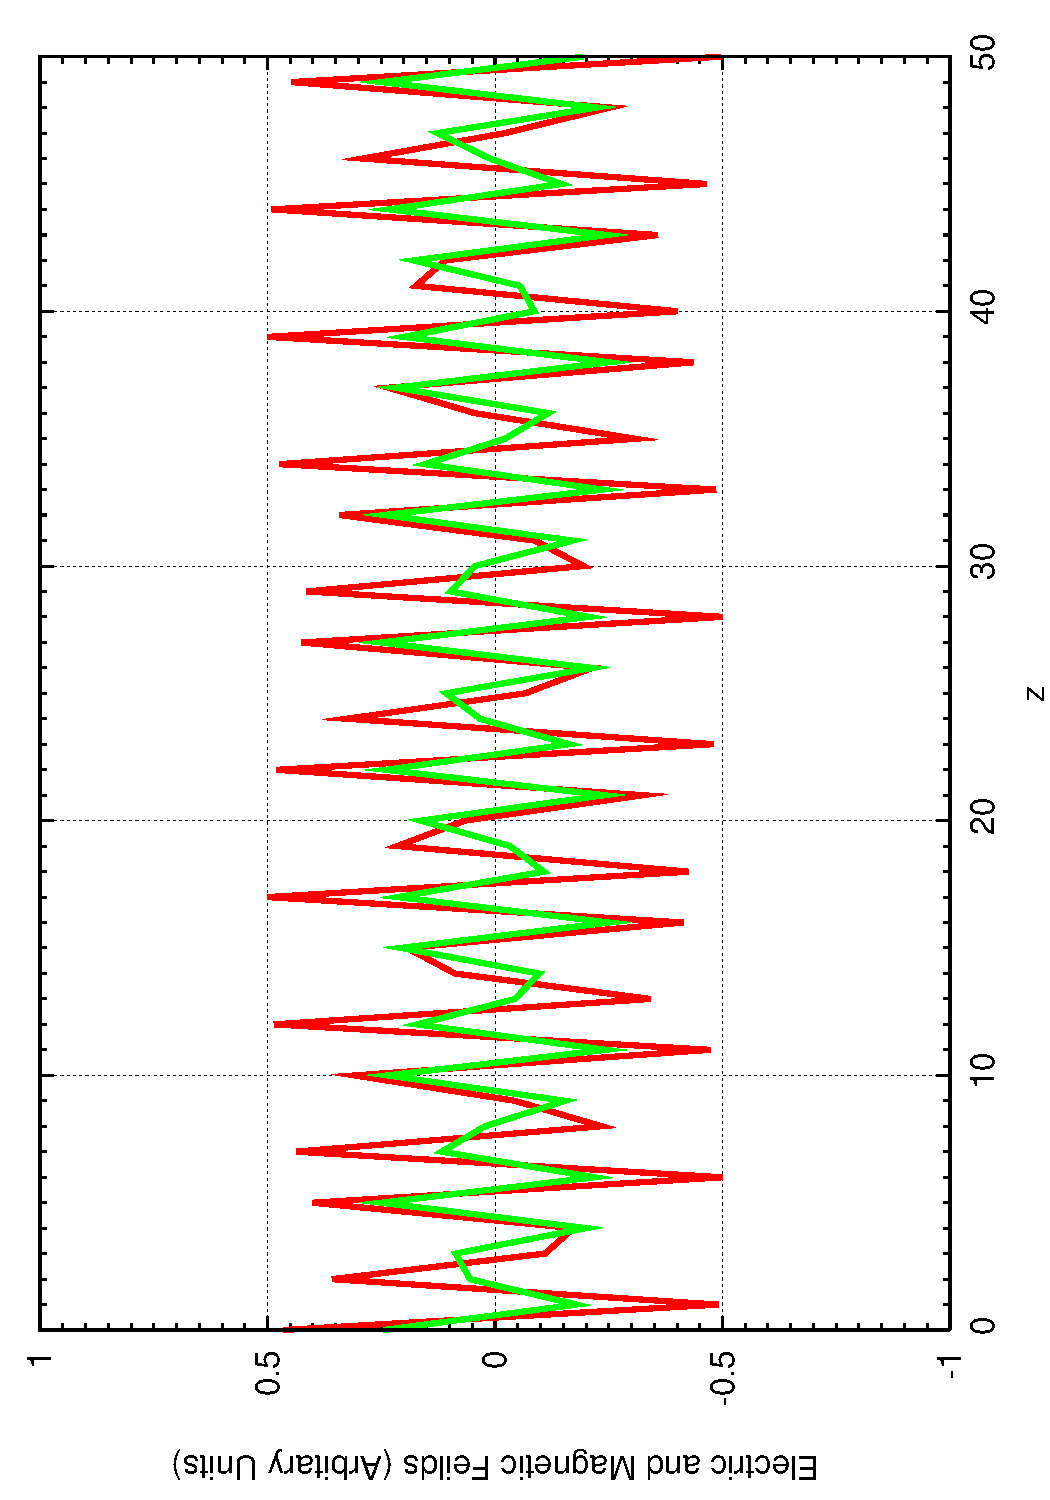
\includegraphics[angle=270, width=\textwidth]{highfreqsine4.pdf}
        \end{subfigure}
        \caption{The effect of aliasing on the accuracy of the function calculated by the simulation when plotting the function $0.5\sin(ax)$ for increasing $a$. The first two graphs show the wave at the usual resolution as used previously and the second two show the waves for higher frequencies with a shorter $x$ space so that the effect can be seen more clearly.}\label{fig:highfreqsine}
\end{figure}
The Fourier transform of a Gaussian represents the function in frequency space. For the function defined in equation \ref{eq:gaussian}, the Fourier transform is $\mathcal{F}_x$. This is also a Gaussian function, as shown in figure \ref{fig:fouriergauss}.
\begin{align}
        \mathcal{F}_x \left[\e{-ax^2}\right] (k) &= \int_{-\infty}^{\infty} \e{-ax^2}\e{-2\pi ikx}\D{x} \\
        &= \int_{-\infty}^{\infty} \e{-ax^2} \Big[\cos(2\pi kx)-i\sin(2\pi kx)\Big]\D{x} \\
        &= \int_{-\infty}^{\infty} \e{-ax^2} \cos(2\pi kx) dx -i\int_{-\infty}^{\infty}\sin(2\pi kx)\D{x} 
        \intertext{The second of these equations, $\int\sin(x)\D{x}$, is odd. Any odd function integrated over a symmetrical range is equal to 0, thus only the first integral makes a contribution.}
        \therefore \mathcal{F}_x\Big[\e{-ax^2}\Big](k) &= \sqrt{\frac{\pi}{a}}\e{\frac{-\pi^2 k^2}{a} }
\end{align} 
\begin{figure}[ht]
  \centering
  \begin{overpic}[angle=270, width=0.6\textwidth]{gaussian.pdf}
    \put(60,35){$\mathcal{F}_x(k) = \sqrt{\frac{\pi}{a}}\e{\frac{-\pi^2 k^2}{a} }$}
    \put(60,50){$f(x) = \e{-ax^2}$}
    \put(63,47){\vector(-3,-1){6}}
    \put(70,33){\vector(-3,-4){6}}
  \end{overpic}
  \caption{\label{fig:fouriergauss}The Fourier transform of the Gaussian function is also a Gaussian with a larger range of frequencies..}
\end{figure}

One of the effects of a dielectric is to separate out the frequencies in a travelling wave, since they move at different velocities in the material. This is the effect that is observed here. Since the Fourier transform shows that the frequencies are more widely spread, this happens to a greater degree the higher the frequency being modelled. 

This property means that unless the function is calculated to infinite precision, there will be some frequencies left out, and so not a perfect wave. This is the phenomenon that is taking place when the wave enters the dielectric material. When it enters the material, the wavelength gets shorter and so the frequency increases. This means that the high frequencies that make up the Gaussian function are also increased and since the simulation has a high temporal/spacial step, this causes the same aliasing as seen in figure \ref{fig:highfreqsine}.

In order to correct this, or at least reduce its effect, the relative spacial/temporal step can be reduced. This means that there are more points calculated for the fields per unit length of the simulation area and so a greater accuracy of the results. When the spacial resolution is increased, there are naturally compromises in the time taken to calculate each frame. In figure \ref{fig:highresolutuion1}, the size of the grid is changed from 200 nodes wide, to 2000 nodes wide. This has the effect of narrowing all of the function's appearance since they are all still calculated with optimisation of the previous width. Instead, the functions are changed so that they reflect the increase in width. This means that the function being plotted is in fact a different function, but since this represents only a scaling factor, and since the system has been scaled by the same factor, there is no difference in the observed behaviour.

\begin{figure}[ht]
        \centering
        \begin{subfigure}[ht]{0.45\textwidth}
                \centering
                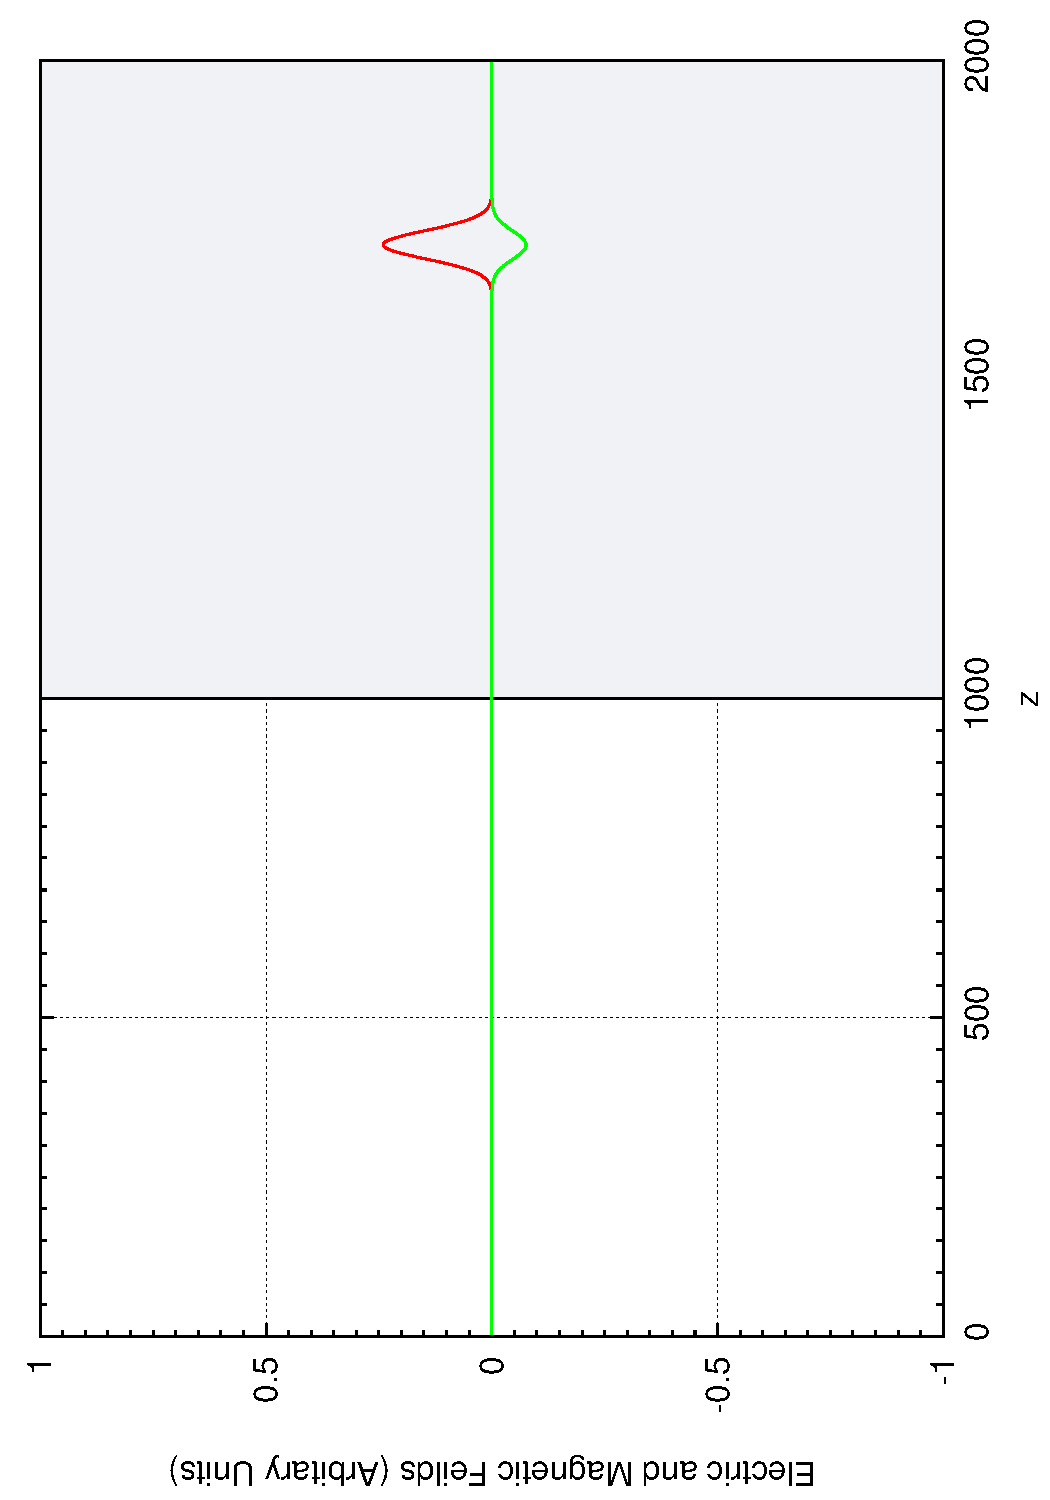
\includegraphics[angle=270, width=\textwidth]{gaussnoise2.pdf}
        \end{subfigure}%
        ~
        \begin{subfigure}[ht]{0.45\textwidth}
                \centering
                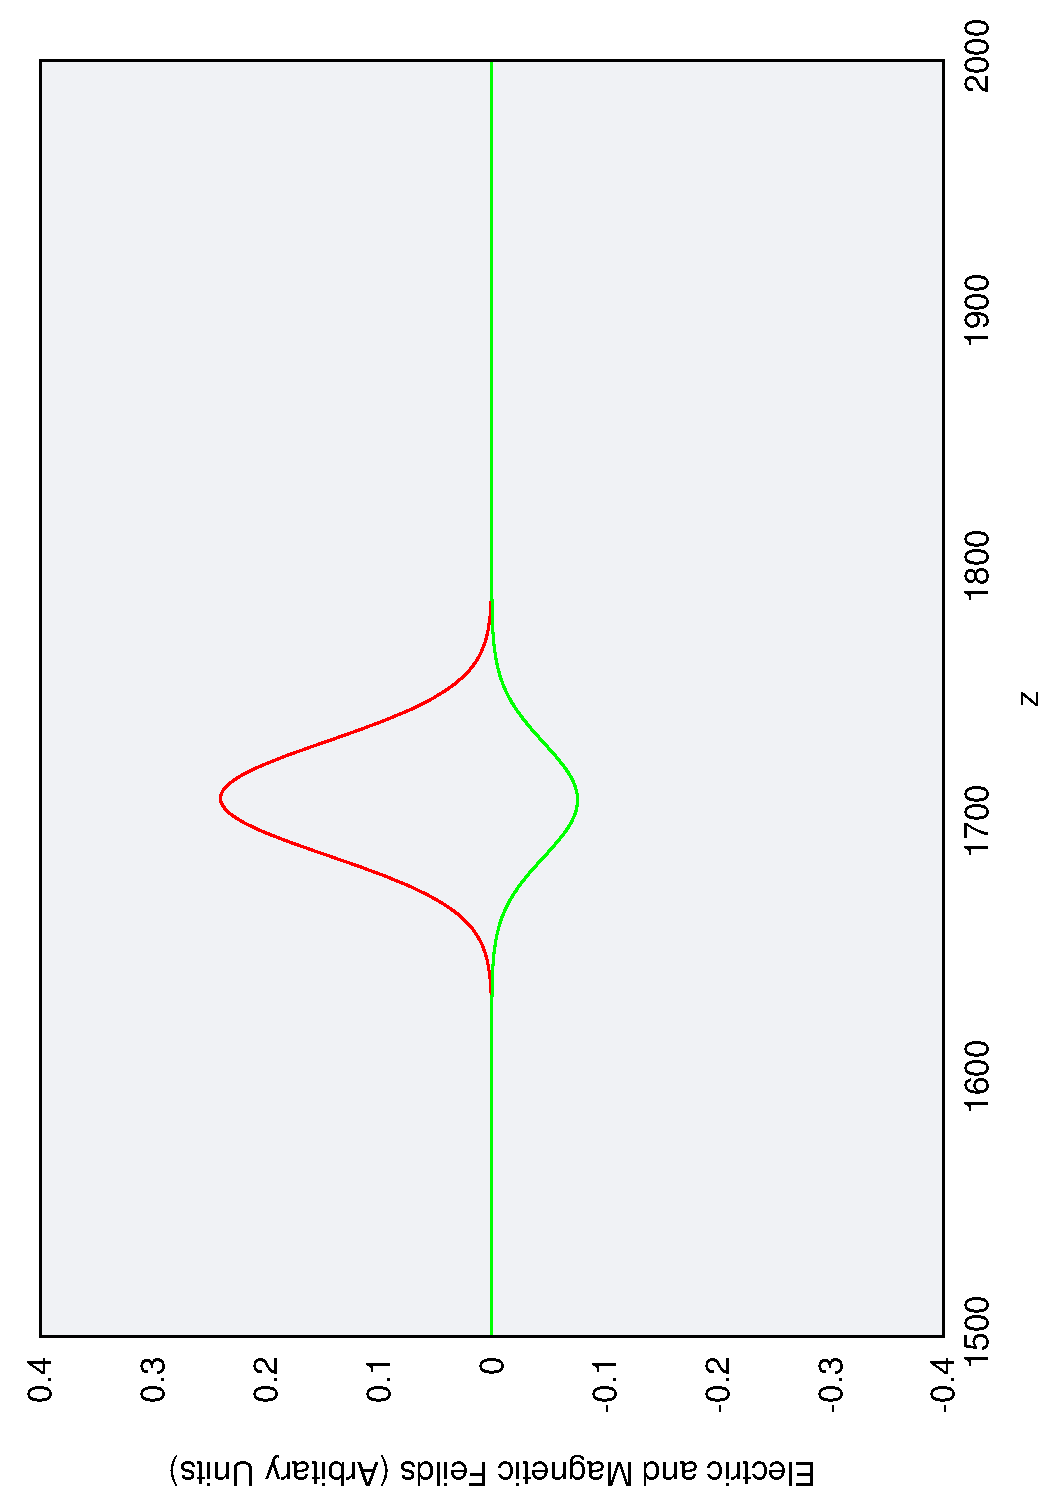
\includegraphics[angle=270, width=\textwidth]{gaussnoise2b.pdf}
        \end{subfigure}
        \caption{Two frames from a wave that is created in the centre of the region. The seed point creates two pulses that move away from each other. The amplitude is set to one half of previous so that when they interact after colliding with the walls, the resulting peak stays within the graphing area.}\label{fig:highresolutuion1}
\end{figure}
% subsubsection non_lossy_material (end)

\subsubsection{Lossy Material} % (fold)
\label{ssub:lossy_material}
A dielectric with a finite permittivity is simple to demonstrate since there is no change in the wave once it has entered the dielectric material. The only change to the wave is at the boundary, it is a homogeneous material. Instead, it is possible to add a loss factor to the dielectric so that the medium shows some inhomogeneity.

This is done by simply applying a scaling factor, or finite conductivity, on the wave which is dependant on the position in the dielectric as the wave moves through it. A conduction-current term can be added to the equation used to start with, equation \ref{eq:max2}, as shown in equation \ref{eq:conductioncurrent}.
\begin{align}
    \curl{\vec{H}} &= \epsilon \pd{\vec{E}}{t} + \sigma \vec{E}\label{eq:conductioncurrent} 
    \intertext{This can be reduced to the single dimension as before and written in terms of the variable part of the function}
    \dx{H_y}{x} &= \epsilon \dx{E_z}{t} + \sigma E_z
    \intertext{This equation can then be discretized for use with the FDTD algorithm so that the update equations become}
    \frac{H(m+\frac{1}{2})-H(m-\frac{1}{2})}{\delta} &= \epsilon \frac{E(m+1)-E(m)}{\delta} + \sigma \frac{E(m+1)+E(m)}{2}
\end{align}

The final term is the finite conductivity. This form is used as it is the time average of the electric field nodes at the points $m$ and $(m+1)$, since there is no node at the point $(m+\frac{1}{2})$.

When such a material is added to the simulation region, there is no change to the reflection coefficient, or the shape of the wave when first it enters the dielectric, compared to if the dielectric was not lossy. The only change that is observed is to the amplitude of the wave which slowly decreases as it moves through the material. Figure \ref{fig:lossydiele} shows several stages of the wave as it is moving through the dielectric.

\begin{figure}[ht]
    \centering
    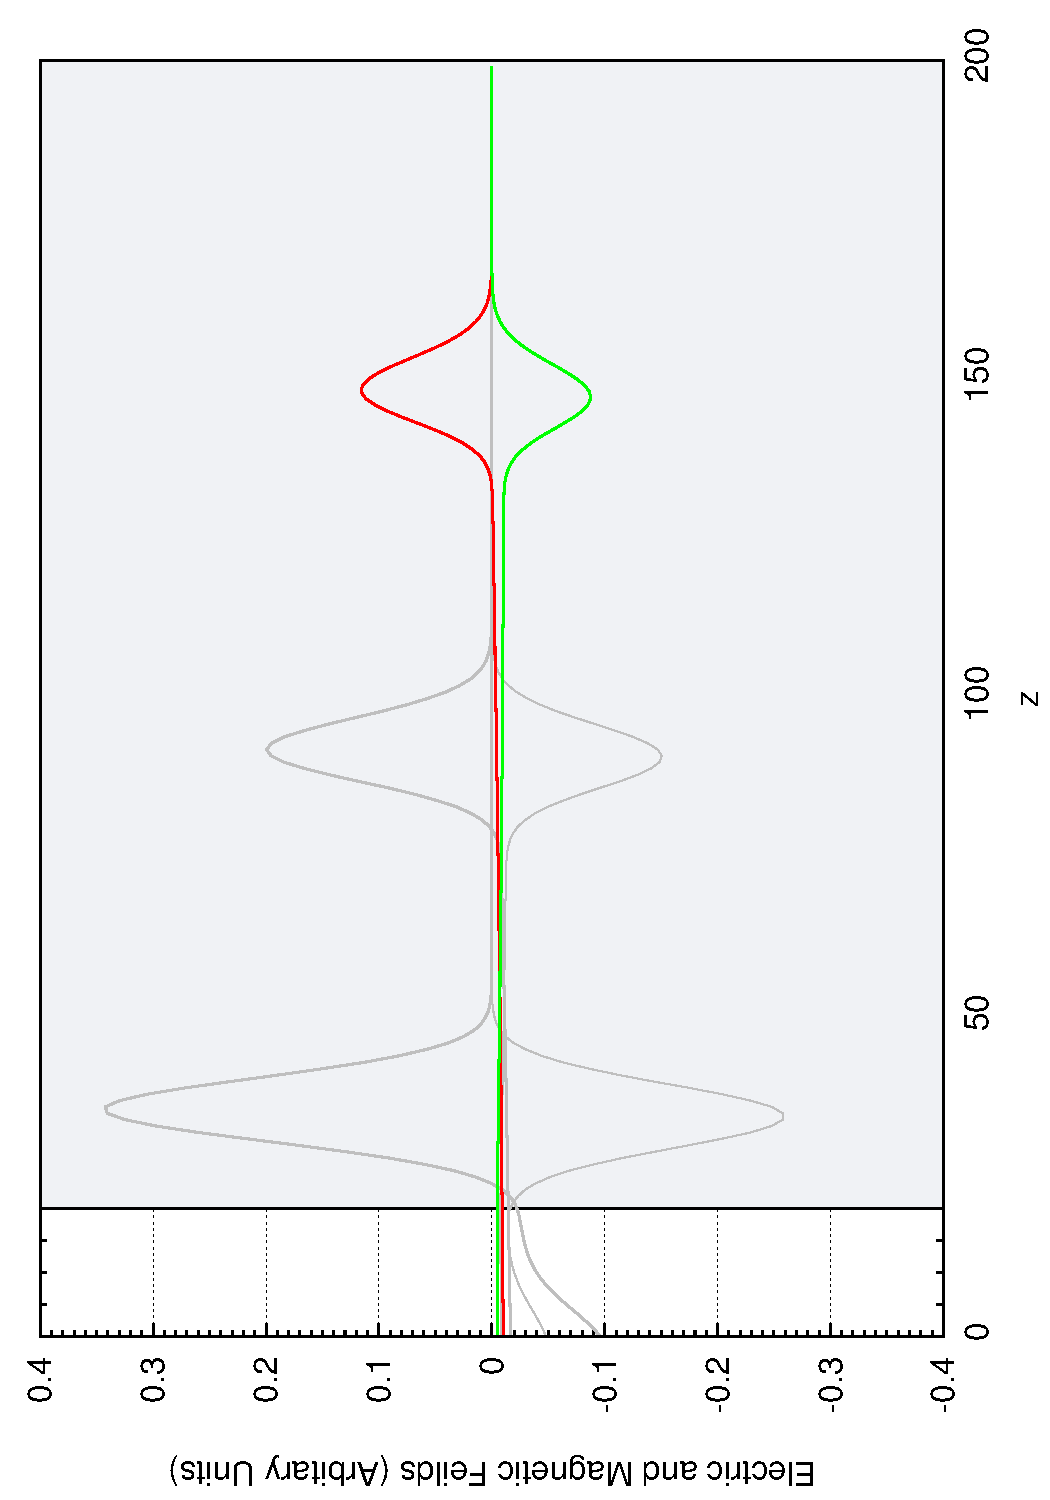
\includegraphics[angle=270, width=0.6\textwidth]{lossydielec1.pdf}
    \caption{Several frames showing the wave after it has entered the dielectric material. Each image is 80 frames apart. The lossyness of the dielectric has been set to 0.01 which means that each the amplitude of the wave is 99\% of its previous value for each step of the simulation .}\label{fig:lossydiele}
\end{figure}
% subsubsection lossy_material (end)
% subsection dielectirc_material (end)

\subsection{Total Field/Scattered Field Boundary} % (fold)
\label{sub:total_field_scattered_field_boundary}
So far, the only types of sources that have been modelled are the fixed and the additive source. These both result in a wave that is created at a single static point, and travels in both directions away from the source. But it is possible to initiate a wave such that it moves only in a single direction. We shall consider the case of a wave created and moving in the positive direction, from left to right, a very similar approach is needed for the opposite case. This is possible using a total field/scattered field boundary (TFSF). This is coded as simply the original field that is created moving in both directions, with an extra step that simply removes the magnitude of the wave from the direction that is not desired. 

So, for this example, a step that takes the Gaussian function away from the node on the left side of the source is added. This results in a wave that travels in only one direction. The TFSF method is similar to the total absorbing boundary we saw previously, that allowed the simulation area to be more than a confined box, but to extend to infinity. The difference here is that the wave is generated at this point, but if it were to be reflected back from a boundary and re-encounter this point, it would be able to travel through the source node as if it were any other node. An implementation  of the TFSF is shown in figure \ref{fig:TFSF}, which also shows the same wave after it has been incident on a dielectric boundary and passed through the same source node again.

\begin{figure}[ht]
        \centering
        \begin{subfigure}[ht]{0.45\textwidth}
                \centering
                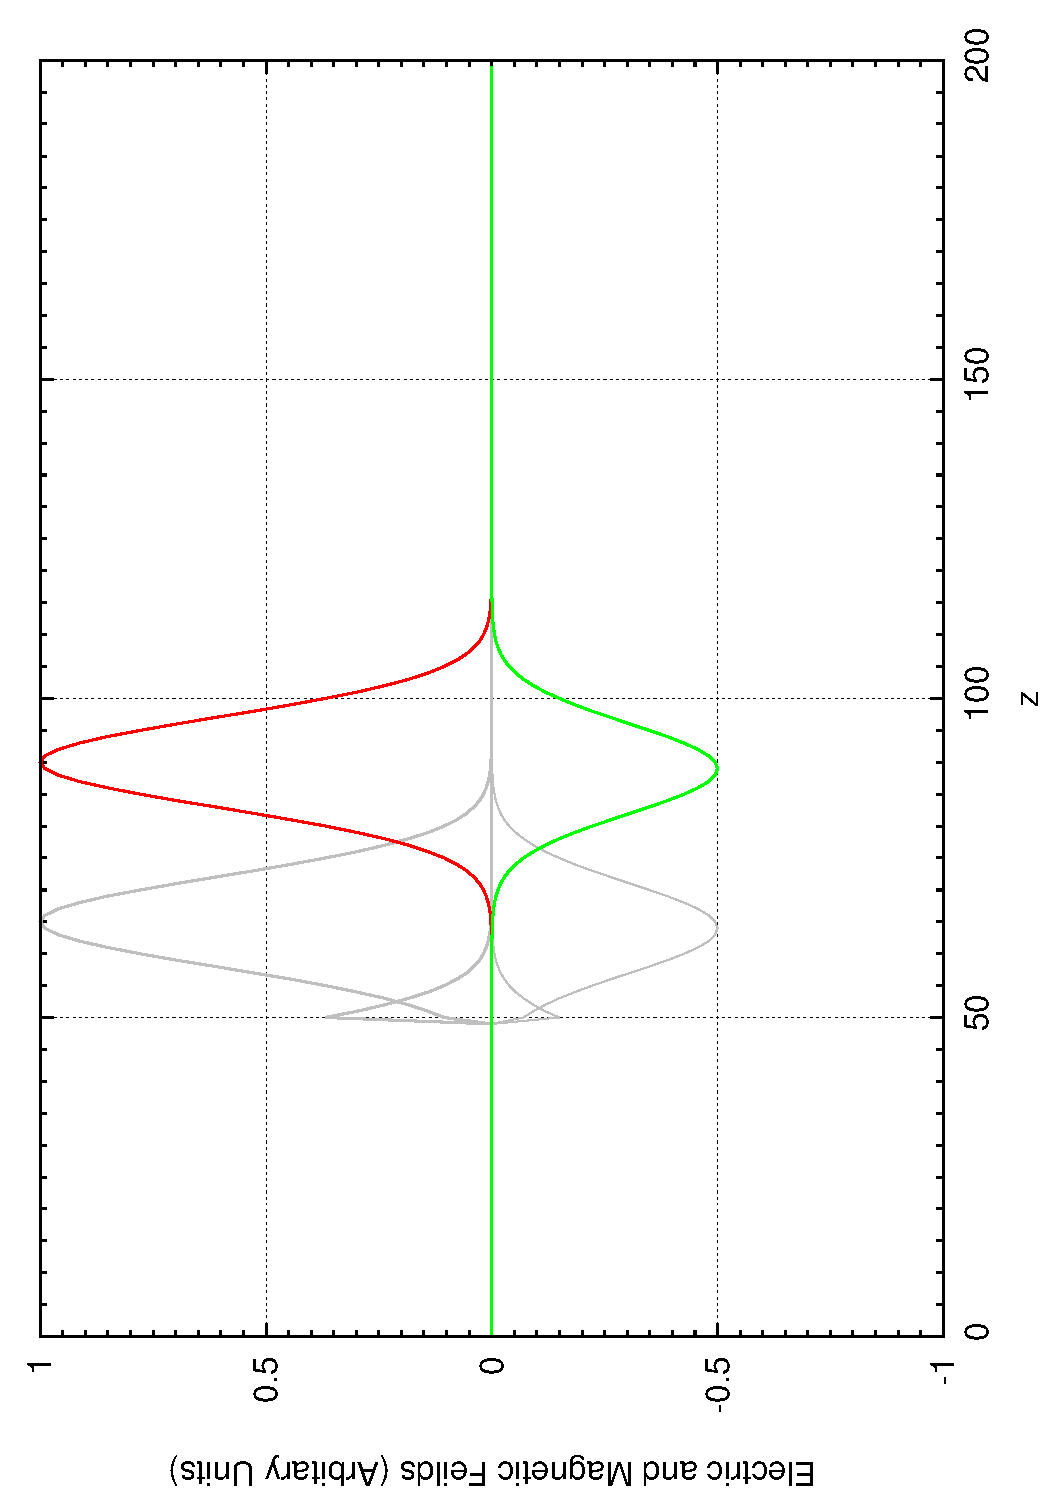
\includegraphics[angle=270, width=\textwidth]{TFSF1.pdf}
        \end{subfigure}%
        ~
        \begin{subfigure}[ht]{0.45\textwidth}
                \centering
                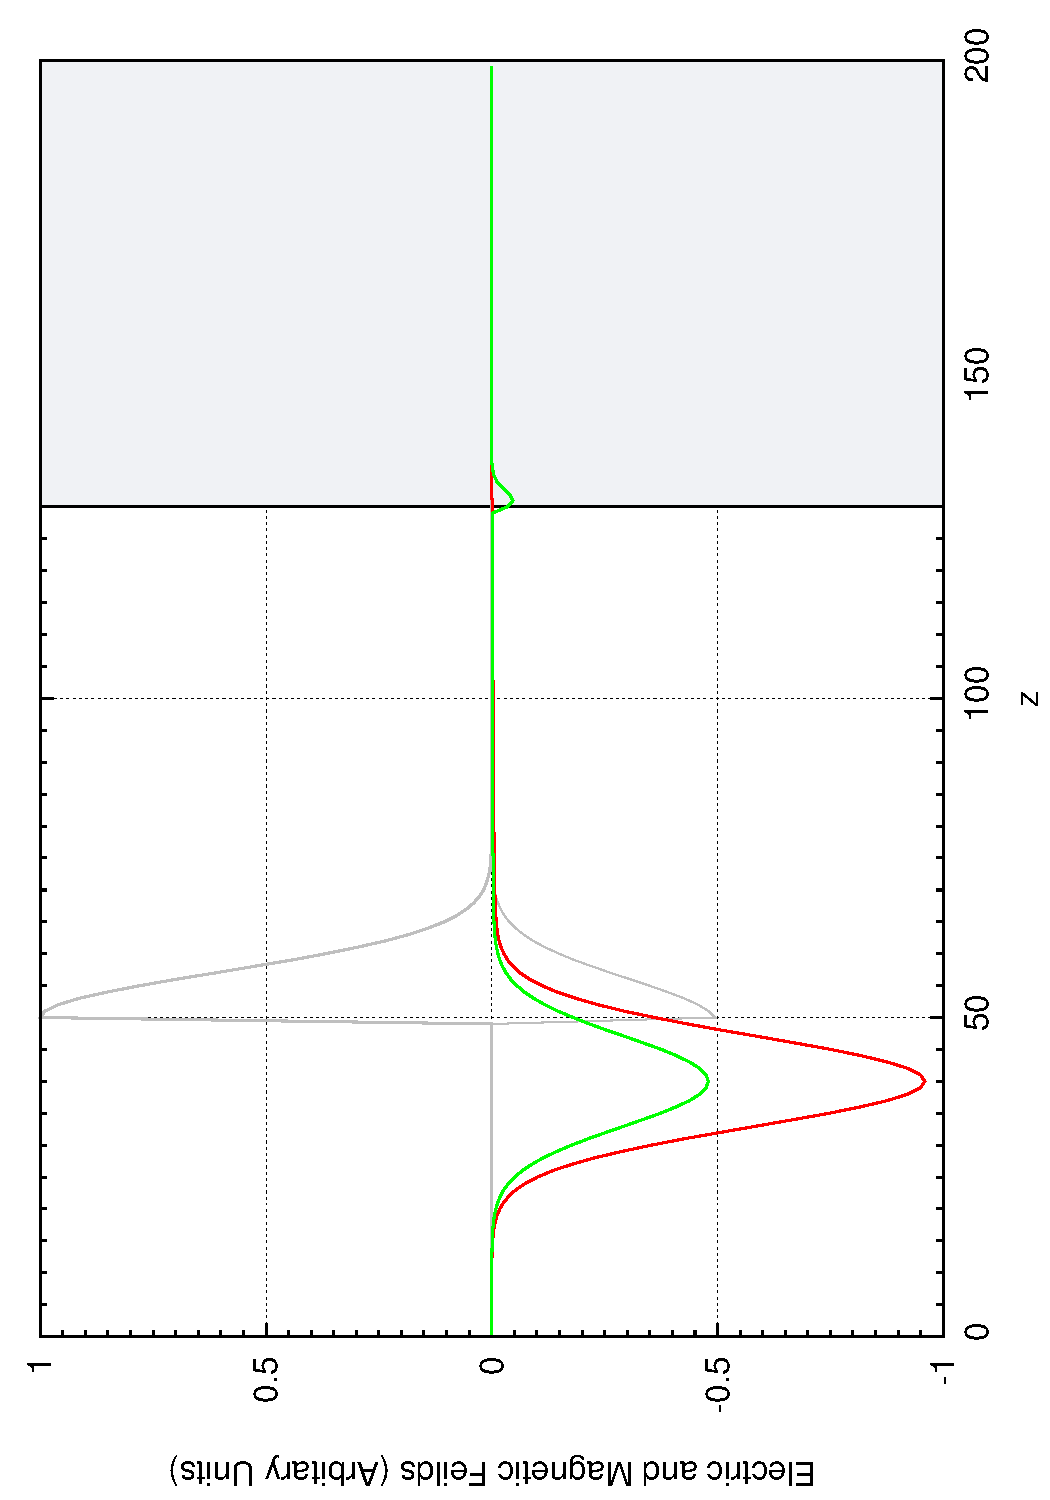
\includegraphics[angle=270, width=\textwidth]{TFSF2.pdf}
        \end{subfigure}
        \caption{Several frame showing the creation and resulting propagation of a wave created at a TFSF boundary, as well as a frame showing how the TFSF boundary acts like a regular node when the wave is reflected from a dielectric boundary and passes through the initial source point.}\label{fig:TFSF}
\end{figure}

The TFSF boundary gets its name from the resulting behaviour of the simulation area. Once a TFSF boundary is created, the area is separated into two distinct regions (again we shall consider only the case for the wave generated at the source and moving right). The right is the Total Field, the left is the Scattered Field. The source creates a wave that only exists in the total field initially, it is only if the wave encounters a boundary and scatters from it that it is able to reach the scattered field region.


% subsection total_field_scattered_field_boundary (end)

% section simulations (end)

%!TEX root = main.tex

\section{Shortcomings} % (fold)
\label{sec:shortcomings}
The finite difference time domain method is very good at approximating systems such as an electromagnetic wave. However there are a few areas where the model does not perform completely accurately. 

\subsection{Grid Size} % (fold)
\label{sub:grid_size}
The accuracy of the simulation depends both on the equations and approximations used in the mathematical representation of the wave and on the grid used to model and calculate that wave. The default size of the grid used here is 200 nodes long. That is, there are 200 electric field nodes and 200 magnetic field nodes used to calculate the field. Increasing this number would improve the accuracy and remove some of the artefacts shown previously. However, to do so would increase the time and processor load required for each simulation. This is a compromise that can be improved by optimising the code to take advantage of modern computing such as parallel computing and multi threaded calculations. These features are outside the scope of my knowledge.
% subsection grid_size (end)

\subsection{Ambiguous Dielectric Boundary} % (fold)
\label{sub:ambiguous_dielectric_boundary}

One example is when the wave encounters a dielectric boundary and is partially reflected from it. Consider the image in figure \ref{fig:magneticgain}.

\begin{figure}[ht]
    \centering
    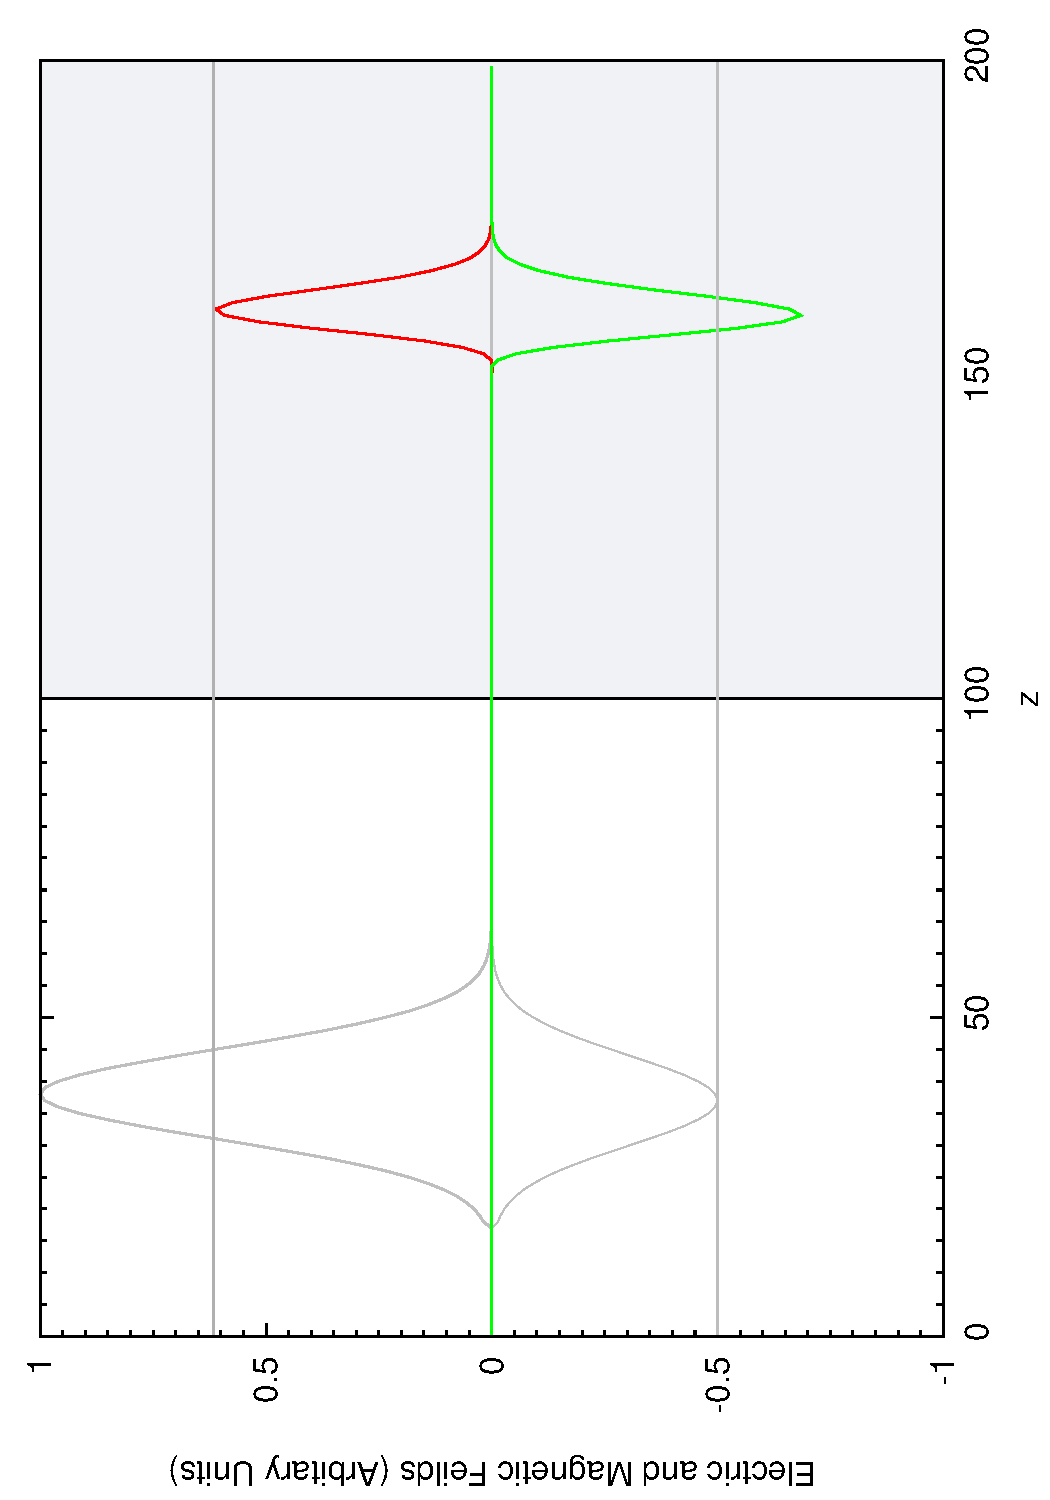
\includegraphics[angle=270, width=0.6\textwidth]{magneticgain.pdf}
    \caption{Several frames showing the wave after it has entered the dielectric material. Each image is 80 frames apart. The lossyness of the dielectric has been set to 0.01 which means the amplitude of the wave is 99\% of its previous value for each step of the simulation .}\label{fig:magneticgain}
\end{figure}

For this simulation, the lossy-less of the dielectric has been set to zero and a permittivity of 5.0 set. As can be seen, the electric field is reduced as would be expected. The magnetic field, however, has increased in magnitude since passing through the boundary. This does not make physical sense since the combined magnitude of the reflected (not shown) and the transmitted wave would be greater than the initial incident wave. This means that some energy has been added to the system despite no external source being present.

The reason for this discrepancy lies in the way that the nodes are arranged that make up the simulation area. There exist nodes that govern the size of the electric field and separate nodes for the magnetic field. These are arranged such that they alternate magnetic-electric-magnetic. This means that the boundary between the dielectric material and free space is not definite but somewhat ambiguous, as shown in figure \ref{fig:dielectricnodes}.

\begin{figure}[ht]
	\centering
	\begin{tikzpicture}
		\node (electric) at (4,2) {Electric Field Nodes};
		\draw [<->] (3,2.5) -- (5,2.5);
		\node (electric) at (4,-2) {Magnetic Field Nodes};
		\draw [<->] (3,-2.5) -- (5,-2.5);
		\node (electric) at (2.5,1.5) {No Dielectric};
		\draw [<-] (0,1.5) -- (1,1.5);
		\node (magnetic) at (5,1.5) {Dielectric};
		\draw [->] (6,1.5) -- (7,1.5);
		\node (1) at (0,0) {$E_z$};
		\node (2) at (1,0) {$H_y$};
		\node (3) at (2,0) {$E_z$};
		\node (4) at (3,0) {$H_y$};
		\node (5) at (4,0) {$E_z$};
		\node (6) at (5,0) {$H_y$};
		\node (7) at (6,0) {$E_z$};
		\node (8) at (7,0) {$H_y$};
		\node (9) at (8,0) {$E_z$};
		\node (10) at (9,0) {$H_y$};
		\draw [fill=darkgray] (-1,1) -- (2,1) -- (2,0.5) -- (-1,0.5);
		\draw [fill=darkgray] (0,1) -- (2,1) -- (2,0.5) -- (0,0.5) -- cycle;
		\draw [fill=darkgray] (2,1) -- (4,1) -- (4,0.5) -- (2,0.5) -- cycle;
		\draw (4,1) -- (6,1) -- (6,0.5) -- (4,0.5) -- cycle;
		\draw (6,1) -- (8,1) -- (8,0.5) -- (6,0.5) -- cycle;
		\draw (8,1) -- (10,1) -- (10,0.5) -- (8,0.5) -- cycle;
		\draw [fill=darkgray] (-1,-1) -- (1,-1) -- (1,-0.5) -- (-1,-0.5) -- cycle;
		\draw [fill=darkgray] (1,-1) -- (3,-1) -- (3,-0.5) -- (1,-0.5) -- cycle;
		\draw [fill=lightgray] (3,-1) -- (5,-1) -- (5,-0.5) -- (3,-0.5) -- cycle;
		\draw (5,-1) -- (7,-1) -- (7,-0.5) -- (5,-0.5) -- cycle;
		\draw (7,-1) -- (9,-1) -- (9,-0.5) -- (7,-0.5) -- cycle;
		\draw (10,-0.5) -- (9,-0.5) -- (9,-1) -- (10,-1);
		\draw [dashed] (4,1.5) -- (4,-1.5);
		\node (magnetic) at (7,-1.5) {Ambiguous node};
		\draw [->] (5.3,-1.4) -- (4.5,-1.1);
	\end{tikzpicture}
	\caption{Arrangement of the nodes that are used to calculate the evolution of the electric and magnetic fields and the ambiguity because of this when a dielectric is modelled.\label{fig:dielectricnodes}}
\end{figure}

When the simulation is run, using this arrangement of nodes, the boundary causes these irregularities to start, in the form of strange behaviour in the way the update equations are handled. To understand what is happening, we need to consider the individual nodes around the boundary, as shown in figure \ref{fig:dielectricnodes}. As the wave moves towards the dielectric, the leading edge crosses the boundary as the electric field nodes are concerned, and so the relevant equations cause transmitted and reflected waves to be generated in accordance to the properties of the dielectric being modelled. However, the wave has not yet reached the magnetic node that is closest to the boundary. This means that there is a component that exists only as an electric field. Clearly this is non physical since the electric and magnetic field essentially generate each other, but the simulation exists in this state for a finite time.

When the wave encounters the magnetic field, the update equations use the value from the corresponding electric field node to calculate the magnetic field, but since the electric field is greater at that point than would be expected, the resulting magnetic field is also greater than expected. As the wave continues into the dielectric material, the calculations continue as usual, but with this error included. Over the length of the wave, i.e.\ the time it takes to move entirely into the dielectric and create the resulting reflected wave, the effect of the initial error is exaggerated so that the magnetic field ends up growing to larger than its initial value. The size of this effect is dependant on the characteristics of the dielectric, but is generally of the order of 1.3 to 1.6 times larger.

The best way to overcome this problem would be to have the dielectric boundary lie exactly on an electric and a magnetic field node. Unfortunately this would require the number of nodes to be increased hugely resulting in impractical calculation times and processor load. Alternatively, the electric and magnetic nodes could be placed at the same spacial position so that a boundary could be placed covering both, simply by placing it at a point where there are two nodes. This however would result in a simulation area that is unable to be used with the finite difference time domain algorithm since there would be no past value of one of the fields that could be used to calculate a further step in time. Other methods do exist, but the FDTD is one of the best in terms of calculation number and flexibility and so others are outside the scope of this report.

A compromise between these idealised situations is more reasonable. Instead of forcing the dielectric boundary to exist only at a single location, and to still be able to apply the FDTD method to the system, the existing set-up can be adapted to make the boundary more ``fuzzy'' but also more symmetrical so that there is less danger of these sorts of errors developing. If the boundary point is treated as the average of the two nodes on either side, the dielectric will appear to make a more gradual change from free space to a finite permittivity. This is done by replacing the absolute definition of the permittivity across the boundary with one that takes into account this difference in location, as shown in equation \ref{eq:averagedielec}.
\begin{align}
	E^{q+\frac{1}{2}}_z(m) &\approx \frac{E^{q+1}_z(m)+E^q_z(m)}{2} \label{eq:averagedielec}
\end{align}
% subsection ambiguous_dielectric_boundary (end)

\subsection{Dimensional Constraints} % (fold)
\label{sub:dimensional_constraints}
Finally, an obvious shortcoming of this model is that it represents only the single $z$ dimension. For real world purposes, the full three dimensions would be required. This would require generalising the update equations from section \ref{sub:finite_differences}
% subsection dimensional_constraints (end)
% section shortcomings (end)

\section{Conclusion} % (fold)
\label{sec:conclusion}
This project was designed to investigate and build a program to implement the finite difference time domain algorithm to calculate an electromagnetic wave as it interacted with different systems. The program allows the setting of a system with definable boundaries, and the ability to add a dielectric and change the lossyness and relative permittivity of that dielectric and also the option to model different starting waves, from a single Gaussian to a travelling sine wave as well as a finite sinusoidal wave pulse and to initiate that wave from either a single static source, or use a TFSF boundary.

The FDTD method is an extremely powerful method for modelling a system of differential equations. This program implements only a very small number of features that would be possible using the mathematical representation of the waves. There are also numerous improvements that could be made regarding the code quality, techniques and efficiency, since to model more complex systems would increase the number of calculations and so the processor load required dramatically.

Overall, however, this program is successful in implementing an initial trial of the FDTD method, incorporating Yee's algorithm.
% section conclusion (end)



\end{document}
